
\documentclass{article} % For LaTeX2e
\usepackage{iclr2024_conference,times}

% Optional math commands from https://github.com/goodfeli/dlbook_notation.
%%%%% NEW MATH DEFINITIONS %%%%%

\usepackage{amsmath,amsfonts,bm}

% Mark sections of captions for referring to divisions of figures
\newcommand{\figleft}{{\em (Left)}}
\newcommand{\figcenter}{{\em (Center)}}
\newcommand{\figright}{{\em (Right)}}
\newcommand{\figtop}{{\em (Top)}}
\newcommand{\figbottom}{{\em (Bottom)}}
\newcommand{\captiona}{{\em (a)}}
\newcommand{\captionb}{{\em (b)}}
\newcommand{\captionc}{{\em (c)}}
\newcommand{\captiond}{{\em (d)}}

% Highlight a newly defined term
\newcommand{\newterm}[1]{{\bf #1}}


% Figure reference, lower-case.
\def\figref#1{figure~\ref{#1}}
% Figure reference, capital. For start of sentence
\def\Figref#1{Figure~\ref{#1}}
\def\twofigref#1#2{figures \ref{#1} and \ref{#2}}
\def\quadfigref#1#2#3#4{figures \ref{#1}, \ref{#2}, \ref{#3} and \ref{#4}}
% Section reference, lower-case.
\def\secref#1{section~\ref{#1}}
% Section reference, capital.
\def\Secref#1{Section~\ref{#1}}
% Reference to two sections.
\def\twosecrefs#1#2{sections \ref{#1} and \ref{#2}}
% Reference to three sections.
\def\secrefs#1#2#3{sections \ref{#1}, \ref{#2} and \ref{#3}}
% Reference to an equation, lower-case.
\def\eqref#1{equation~\ref{#1}}
% Reference to an equation, upper case
\def\Eqref#1{Equation~\ref{#1}}
% A raw reference to an equation---avoid using if possible
\def\plaineqref#1{\ref{#1}}
% Reference to a chapter, lower-case.
\def\chapref#1{chapter~\ref{#1}}
% Reference to an equation, upper case.
\def\Chapref#1{Chapter~\ref{#1}}
% Reference to a range of chapters
\def\rangechapref#1#2{chapters\ref{#1}--\ref{#2}}
% Reference to an algorithm, lower-case.
\def\algref#1{algorithm~\ref{#1}}
% Reference to an algorithm, upper case.
\def\Algref#1{Algorithm~\ref{#1}}
\def\twoalgref#1#2{algorithms \ref{#1} and \ref{#2}}
\def\Twoalgref#1#2{Algorithms \ref{#1} and \ref{#2}}
% Reference to a part, lower case
\def\partref#1{part~\ref{#1}}
% Reference to a part, upper case
\def\Partref#1{Part~\ref{#1}}
\def\twopartref#1#2{parts \ref{#1} and \ref{#2}}

\def\ceil#1{\lceil #1 \rceil}
\def\floor#1{\lfloor #1 \rfloor}
\def\1{\bm{1}}
\newcommand{\train}{\mathcal{D}}
\newcommand{\valid}{\mathcal{D_{\mathrm{valid}}}}
\newcommand{\test}{\mathcal{D_{\mathrm{test}}}}

\def\eps{{\epsilon}}


% Random variables
\def\reta{{\textnormal{$\eta$}}}
\def\ra{{\textnormal{a}}}
\def\rb{{\textnormal{b}}}
\def\rc{{\textnormal{c}}}
\def\rd{{\textnormal{d}}}
\def\re{{\textnormal{e}}}
\def\rf{{\textnormal{f}}}
\def\rg{{\textnormal{g}}}
\def\rh{{\textnormal{h}}}
\def\ri{{\textnormal{i}}}
\def\rj{{\textnormal{j}}}
\def\rk{{\textnormal{k}}}
\def\rl{{\textnormal{l}}}
% rm is already a command, just don't name any random variables m
\def\rn{{\textnormal{n}}}
\def\ro{{\textnormal{o}}}
\def\rp{{\textnormal{p}}}
\def\rq{{\textnormal{q}}}
\def\rr{{\textnormal{r}}}
\def\rs{{\textnormal{s}}}
\def\rt{{\textnormal{t}}}
\def\ru{{\textnormal{u}}}
\def\rv{{\textnormal{v}}}
\def\rw{{\textnormal{w}}}
\def\rx{{\textnormal{x}}}
\def\ry{{\textnormal{y}}}
\def\rz{{\textnormal{z}}}

% Random vectors
\def\rvepsilon{{\mathbf{\epsilon}}}
\def\rvtheta{{\mathbf{\theta}}}
\def\rva{{\mathbf{a}}}
\def\rvb{{\mathbf{b}}}
\def\rvc{{\mathbf{c}}}
\def\rvd{{\mathbf{d}}}
\def\rve{{\mathbf{e}}}
\def\rvf{{\mathbf{f}}}
\def\rvg{{\mathbf{g}}}
\def\rvh{{\mathbf{h}}}
\def\rvu{{\mathbf{i}}}
\def\rvj{{\mathbf{j}}}
\def\rvk{{\mathbf{k}}}
\def\rvl{{\mathbf{l}}}
\def\rvm{{\mathbf{m}}}
\def\rvn{{\mathbf{n}}}
\def\rvo{{\mathbf{o}}}
\def\rvp{{\mathbf{p}}}
\def\rvq{{\mathbf{q}}}
\def\rvr{{\mathbf{r}}}
\def\rvs{{\mathbf{s}}}
\def\rvt{{\mathbf{t}}}
\def\rvu{{\mathbf{u}}}
\def\rvv{{\mathbf{v}}}
\def\rvw{{\mathbf{w}}}
\def\rvx{{\mathbf{x}}}
\def\rvy{{\mathbf{y}}}
\def\rvz{{\mathbf{z}}}

% Elements of random vectors
\def\erva{{\textnormal{a}}}
\def\ervb{{\textnormal{b}}}
\def\ervc{{\textnormal{c}}}
\def\ervd{{\textnormal{d}}}
\def\erve{{\textnormal{e}}}
\def\ervf{{\textnormal{f}}}
\def\ervg{{\textnormal{g}}}
\def\ervh{{\textnormal{h}}}
\def\ervi{{\textnormal{i}}}
\def\ervj{{\textnormal{j}}}
\def\ervk{{\textnormal{k}}}
\def\ervl{{\textnormal{l}}}
\def\ervm{{\textnormal{m}}}
\def\ervn{{\textnormal{n}}}
\def\ervo{{\textnormal{o}}}
\def\ervp{{\textnormal{p}}}
\def\ervq{{\textnormal{q}}}
\def\ervr{{\textnormal{r}}}
\def\ervs{{\textnormal{s}}}
\def\ervt{{\textnormal{t}}}
\def\ervu{{\textnormal{u}}}
\def\ervv{{\textnormal{v}}}
\def\ervw{{\textnormal{w}}}
\def\ervx{{\textnormal{x}}}
\def\ervy{{\textnormal{y}}}
\def\ervz{{\textnormal{z}}}

% Random matrices
\def\rmA{{\mathbf{A}}}
\def\rmB{{\mathbf{B}}}
\def\rmC{{\mathbf{C}}}
\def\rmD{{\mathbf{D}}}
\def\rmE{{\mathbf{E}}}
\def\rmF{{\mathbf{F}}}
\def\rmG{{\mathbf{G}}}
\def\rmH{{\mathbf{H}}}
\def\rmI{{\mathbf{I}}}
\def\rmJ{{\mathbf{J}}}
\def\rmK{{\mathbf{K}}}
\def\rmL{{\mathbf{L}}}
\def\rmM{{\mathbf{M}}}
\def\rmN{{\mathbf{N}}}
\def\rmO{{\mathbf{O}}}
\def\rmP{{\mathbf{P}}}
\def\rmQ{{\mathbf{Q}}}
\def\rmR{{\mathbf{R}}}
\def\rmS{{\mathbf{S}}}
\def\rmT{{\mathbf{T}}}
\def\rmU{{\mathbf{U}}}
\def\rmV{{\mathbf{V}}}
\def\rmW{{\mathbf{W}}}
\def\rmX{{\mathbf{X}}}
\def\rmY{{\mathbf{Y}}}
\def\rmZ{{\mathbf{Z}}}

% Elements of random matrices
\def\ermA{{\textnormal{A}}}
\def\ermB{{\textnormal{B}}}
\def\ermC{{\textnormal{C}}}
\def\ermD{{\textnormal{D}}}
\def\ermE{{\textnormal{E}}}
\def\ermF{{\textnormal{F}}}
\def\ermG{{\textnormal{G}}}
\def\ermH{{\textnormal{H}}}
\def\ermI{{\textnormal{I}}}
\def\ermJ{{\textnormal{J}}}
\def\ermK{{\textnormal{K}}}
\def\ermL{{\textnormal{L}}}
\def\ermM{{\textnormal{M}}}
\def\ermN{{\textnormal{N}}}
\def\ermO{{\textnormal{O}}}
\def\ermP{{\textnormal{P}}}
\def\ermQ{{\textnormal{Q}}}
\def\ermR{{\textnormal{R}}}
\def\ermS{{\textnormal{S}}}
\def\ermT{{\textnormal{T}}}
\def\ermU{{\textnormal{U}}}
\def\ermV{{\textnormal{V}}}
\def\ermW{{\textnormal{W}}}
\def\ermX{{\textnormal{X}}}
\def\ermY{{\textnormal{Y}}}
\def\ermZ{{\textnormal{Z}}}

% Vectors
\def\vzero{{\bm{0}}}
\def\vone{{\bm{1}}}
\def\vmu{{\bm{\mu}}}
\def\vtheta{{\bm{\theta}}}
\def\va{{\bm{a}}}
\def\vb{{\bm{b}}}
\def\vc{{\bm{c}}}
\def\vd{{\bm{d}}}
\def\ve{{\bm{e}}}
\def\vf{{\bm{f}}}
\def\vg{{\bm{g}}}
\def\vh{{\bm{h}}}
\def\vi{{\bm{i}}}
\def\vj{{\bm{j}}}
\def\vk{{\bm{k}}}
\def\vl{{\bm{l}}}
\def\vm{{\bm{m}}}
\def\vn{{\bm{n}}}
\def\vo{{\bm{o}}}
\def\vp{{\bm{p}}}
\def\vq{{\bm{q}}}
\def\vr{{\bm{r}}}
\def\vs{{\bm{s}}}
\def\vt{{\bm{t}}}
\def\vu{{\bm{u}}}
\def\vv{{\bm{v}}}
\def\vw{{\bm{w}}}
\def\vx{{\bm{x}}}
\def\vy{{\bm{y}}}
\def\vz{{\bm{z}}}

% Elements of vectors
\def\evalpha{{\alpha}}
\def\evbeta{{\beta}}
\def\evepsilon{{\epsilon}}
\def\evlambda{{\lambda}}
\def\evomega{{\omega}}
\def\evmu{{\mu}}
\def\evpsi{{\psi}}
\def\evsigma{{\sigma}}
\def\evtheta{{\theta}}
\def\eva{{a}}
\def\evb{{b}}
\def\evc{{c}}
\def\evd{{d}}
\def\eve{{e}}
\def\evf{{f}}
\def\evg{{g}}
\def\evh{{h}}
\def\evi{{i}}
\def\evj{{j}}
\def\evk{{k}}
\def\evl{{l}}
\def\evm{{m}}
\def\evn{{n}}
\def\evo{{o}}
\def\evp{{p}}
\def\evq{{q}}
\def\evr{{r}}
\def\evs{{s}}
\def\evt{{t}}
\def\evu{{u}}
\def\evv{{v}}
\def\evw{{w}}
\def\evx{{x}}
\def\evy{{y}}
\def\evz{{z}}

% Matrix
\def\mA{{\bm{A}}}
\def\mB{{\bm{B}}}
\def\mC{{\bm{C}}}
\def\mD{{\bm{D}}}
\def\mE{{\bm{E}}}
\def\mF{{\bm{F}}}
\def\mG{{\bm{G}}}
\def\mH{{\bm{H}}}
\def\mI{{\bm{I}}}
\def\mJ{{\bm{J}}}
\def\mK{{\bm{K}}}
\def\mL{{\bm{L}}}
\def\mM{{\bm{M}}}
\def\mN{{\bm{N}}}
\def\mO{{\bm{O}}}
\def\mP{{\bm{P}}}
\def\mQ{{\bm{Q}}}
\def\mR{{\bm{R}}}
\def\mS{{\bm{S}}}
\def\mT{{\bm{T}}}
\def\mU{{\bm{U}}}
\def\mV{{\bm{V}}}
\def\mW{{\bm{W}}}
\def\mX{{\bm{X}}}
\def\mY{{\bm{Y}}}
\def\mZ{{\bm{Z}}}
\def\mBeta{{\bm{\beta}}}
\def\mPhi{{\bm{\Phi}}}
\def\mLambda{{\bm{\Lambda}}}
\def\mSigma{{\bm{\Sigma}}}

% Tensor
\DeclareMathAlphabet{\mathsfit}{\encodingdefault}{\sfdefault}{m}{sl}
\SetMathAlphabet{\mathsfit}{bold}{\encodingdefault}{\sfdefault}{bx}{n}
\newcommand{\tens}[1]{\bm{\mathsfit{#1}}}
\def\tA{{\tens{A}}}
\def\tB{{\tens{B}}}
\def\tC{{\tens{C}}}
\def\tD{{\tens{D}}}
\def\tE{{\tens{E}}}
\def\tF{{\tens{F}}}
\def\tG{{\tens{G}}}
\def\tH{{\tens{H}}}
\def\tI{{\tens{I}}}
\def\tJ{{\tens{J}}}
\def\tK{{\tens{K}}}
\def\tL{{\tens{L}}}
\def\tM{{\tens{M}}}
\def\tN{{\tens{N}}}
\def\tO{{\tens{O}}}
\def\tP{{\tens{P}}}
\def\tQ{{\tens{Q}}}
\def\tR{{\tens{R}}}
\def\tS{{\tens{S}}}
\def\tT{{\tens{T}}}
\def\tU{{\tens{U}}}
\def\tV{{\tens{V}}}
\def\tW{{\tens{W}}}
\def\tX{{\tens{X}}}
\def\tY{{\tens{Y}}}
\def\tZ{{\tens{Z}}}


% Graph
\def\gA{{\mathcal{A}}}
\def\gB{{\mathcal{B}}}
\def\gC{{\mathcal{C}}}
\def\gD{{\mathcal{D}}}
\def\gE{{\mathcal{E}}}
\def\gF{{\mathcal{F}}}
\def\gG{{\mathcal{G}}}
\def\gH{{\mathcal{H}}}
\def\gI{{\mathcal{I}}}
\def\gJ{{\mathcal{J}}}
\def\gK{{\mathcal{K}}}
\def\gL{{\mathcal{L}}}
\def\gM{{\mathcal{M}}}
\def\gN{{\mathcal{N}}}
\def\gO{{\mathcal{O}}}
\def\gP{{\mathcal{P}}}
\def\gQ{{\mathcal{Q}}}
\def\gR{{\mathcal{R}}}
\def\gS{{\mathcal{S}}}
\def\gT{{\mathcal{T}}}
\def\gU{{\mathcal{U}}}
\def\gV{{\mathcal{V}}}
\def\gW{{\mathcal{W}}}
\def\gX{{\mathcal{X}}}
\def\gY{{\mathcal{Y}}}
\def\gZ{{\mathcal{Z}}}

% Sets
\def\sA{{\mathbb{A}}}
\def\sB{{\mathbb{B}}}
\def\sC{{\mathbb{C}}}
\def\sD{{\mathbb{D}}}
% Don't use a set called E, because this would be the same as our symbol
% for expectation.
\def\sF{{\mathbb{F}}}
\def\sG{{\mathbb{G}}}
\def\sH{{\mathbb{H}}}
\def\sI{{\mathbb{I}}}
\def\sJ{{\mathbb{J}}}
\def\sK{{\mathbb{K}}}
\def\sL{{\mathbb{L}}}
\def\sM{{\mathbb{M}}}
\def\sN{{\mathbb{N}}}
\def\sO{{\mathbb{O}}}
\def\sP{{\mathbb{P}}}
\def\sQ{{\mathbb{Q}}}
\def\sR{{\mathbb{R}}}
\def\sS{{\mathbb{S}}}
\def\sT{{\mathbb{T}}}
\def\sU{{\mathbb{U}}}
\def\sV{{\mathbb{V}}}
\def\sW{{\mathbb{W}}}
\def\sX{{\mathbb{X}}}
\def\sY{{\mathbb{Y}}}
\def\sZ{{\mathbb{Z}}}

% Entries of a matrix
\def\emLambda{{\Lambda}}
\def\emA{{A}}
\def\emB{{B}}
\def\emC{{C}}
\def\emD{{D}}
\def\emE{{E}}
\def\emF{{F}}
\def\emG{{G}}
\def\emH{{H}}
\def\emI{{I}}
\def\emJ{{J}}
\def\emK{{K}}
\def\emL{{L}}
\def\emM{{M}}
\def\emN{{N}}
\def\emO{{O}}
\def\emP{{P}}
\def\emQ{{Q}}
\def\emR{{R}}
\def\emS{{S}}
\def\emT{{T}}
\def\emU{{U}}
\def\emV{{V}}
\def\emW{{W}}
\def\emX{{X}}
\def\emY{{Y}}
\def\emZ{{Z}}
\def\emSigma{{\Sigma}}

% entries of a tensor
% Same font as tensor, without \bm wrapper
\newcommand{\etens}[1]{\mathsfit{#1}}
\def\etLambda{{\etens{\Lambda}}}
\def\etA{{\etens{A}}}
\def\etB{{\etens{B}}}
\def\etC{{\etens{C}}}
\def\etD{{\etens{D}}}
\def\etE{{\etens{E}}}
\def\etF{{\etens{F}}}
\def\etG{{\etens{G}}}
\def\etH{{\etens{H}}}
\def\etI{{\etens{I}}}
\def\etJ{{\etens{J}}}
\def\etK{{\etens{K}}}
\def\etL{{\etens{L}}}
\def\etM{{\etens{M}}}
\def\etN{{\etens{N}}}
\def\etO{{\etens{O}}}
\def\etP{{\etens{P}}}
\def\etQ{{\etens{Q}}}
\def\etR{{\etens{R}}}
\def\etS{{\etens{S}}}
\def\etT{{\etens{T}}}
\def\etU{{\etens{U}}}
\def\etV{{\etens{V}}}
\def\etW{{\etens{W}}}
\def\etX{{\etens{X}}}
\def\etY{{\etens{Y}}}
\def\etZ{{\etens{Z}}}

% The true underlying data generating distribution
\newcommand{\pdata}{p_{\rm{data}}}
% The empirical distribution defined by the training set
\newcommand{\ptrain}{\hat{p}_{\rm{data}}}
\newcommand{\Ptrain}{\hat{P}_{\rm{data}}}
% The model distribution
\newcommand{\pmodel}{p_{\rm{model}}}
\newcommand{\Pmodel}{P_{\rm{model}}}
\newcommand{\ptildemodel}{\tilde{p}_{\rm{model}}}
% Stochastic autoencoder distributions
\newcommand{\pencode}{p_{\rm{encoder}}}
\newcommand{\pdecode}{p_{\rm{decoder}}}
\newcommand{\precons}{p_{\rm{reconstruct}}}

\newcommand{\laplace}{\mathrm{Laplace}} % Laplace distribution

\newcommand{\E}{\mathbb{E}}
\newcommand{\Ls}{\mathcal{L}}
\newcommand{\R}{\mathbb{R}}
\newcommand{\emp}{\tilde{p}}
\newcommand{\lr}{\alpha}
\newcommand{\reg}{\lambda}
\newcommand{\rect}{\mathrm{rectifier}}
\newcommand{\softmax}{\mathrm{softmax}}
\newcommand{\sigmoid}{\sigma}
\newcommand{\softplus}{\zeta}
\newcommand{\KL}{D_{\mathrm{KL}}}
\newcommand{\Var}{\mathrm{Var}}
\newcommand{\standarderror}{\mathrm{SE}}
\newcommand{\Cov}{\mathrm{Cov}}
% Wolfram Mathworld says $L^2$ is for function spaces and $\ell^2$ is for vectors
% But then they seem to use $L^2$ for vectors throughout the site, and so does
% wikipedia.
\newcommand{\normlzero}{L^0}
\newcommand{\normlone}{L^1}
\newcommand{\normltwo}{L^2}
\newcommand{\normlp}{L^p}
\newcommand{\normmax}{L^\infty}

\newcommand{\parents}{Pa} % See usage in notation.tex. Chosen to match Daphne's book.

\DeclareMathOperator*{\argmax}{arg\,max}
\DeclareMathOperator*{\argmin}{arg\,min}

\DeclareMathOperator{\sign}{sign}
\DeclareMathOperator{\Tr}{Tr}
\let\ab\allowbreak


\usepackage{hyperref}
\usepackage{url}
\usepackage{bbm}  %For indicator
\usepackage{subcaption}

\usepackage{xcolor}

% Define the \TK command
\newcommand{\TK}[1]{\textcolor{red}{TK: #1}}


\title{Language Models as Auction Participants }

% Authors must not appear in the submitted version. They should be hidden
% as long as the \iclrfinalcopy macro remains commented out below.
% Non-anonymous submissions will be rejected without review.

\author{Anand, Kehang \& Yancheng Jiang\thanks{ Use footnote for providing further information
about author (webpage, alternative address)---\emph{not} for acknowledging
funding agencies.  Funding acknowledgements go at the end of the paper.} \\
Department of Computer Science\\
Cranberry-Lemon University\\
Pittsburgh, PA 15213, USA \\
\texttt{\{hippo,brain,jen\}@cs.cranberry-lemon.edu} \\
\And
Ji Q. Ren \& Yevgeny LeNet \\
Department of Computational Neuroscience \\
University of the Witwatersrand \\
Joburg, South Africa \\
\texttt{\{robot,net\}@wits.ac.za} \\
\AND
Coauthor \\
Affiliation \\
Address \\
\texttt{email}
}

% The \author macro works with any number of authors. There are two commands
% used to separate the names and addresses of multiple authors: \And and \AND.
%
% Using \And between authors leaves it to \LaTeX{} to determine where to break
% the lines. Using \AND forces a linebreak at that point. So, if \LaTeX{}
% puts 3 of 4 authors names on the first line, and the last on the second
% line, try using \AND instead of \And before the third author name.

\newcommand{\fix}{\marginpar{FIX}}
\newcommand{\new}{\marginpar{NEW}}

%\iclrfinalcopy % Uncomment for camera-ready version, but NOT for submission.
\begin{document}

\maketitle

\begin{abstract}
This paper investigates auction behavior of simulated AI agents (large language models, or LLMs). 
We begin by benchmarking these LLM-driven agents against established lab experiments across various auction settings: independent private value, affiliated private value, and common value auctions. 
Our findings reveal that LLM agents exhibit many behavioral traits similar to those observed in human participants within lab environments.
Building on this, we investigate multi-unit combinatorial auctions under three distinct bid formats: simultaneous, sequential, and menu-based. 
Our study contributes fresh empirical insights into this classical auction framework.
We run 1,000+ auctions for less than \$100 with GPT-4, and develop a framework flexible enough to run auction experiments with any LLM model and a wide range of mechanism  specification. 

% This paper investigates auction behavior through the lens of three distinct agents: {\em homo economicus} (theoretical predictions), real humans (existing empirical/experimental evidence), and {\em homo silicus} (simulated agents using large language models, or LLMs). We run auction experiments with LLMs in different settings: independent private value, affiliated private value, and common value. First, we show LLM agents fail revenue equivalence due to risk aversion in independent private value settings (echoing existing empirical results). Second, we show LLMs are `better' at playing clock auctions in affiliated private value settings (echoing results on obvious strategyproofness). Third, we demonstrate the presence of the winner's curse in common value settings, with the curse having an increasing bite in larger auctions (echoing \cite{kagel1986winner}). All these results hold for single-unit settings. We also explore multi-unit combinatorial auctions under three bid formats -- simultaneous, sequential, and menu -- to observe how LLMs deal with complements. For robustness, we employ two distinct prompt sets (technical and story-telling) for all experiments and find our results are practically the same under this prompt variation. We run 1,000+ auctions for less than \$100 with GPT-4o, and develop a framework flexible enough to run auction experiments with any LLM model and almost any reasonable prompt specification. 
\end{abstract}

\section{Introduction}
The field of mechanism design, auction theory in particular, has benefited enormously from a rich interplay between empirics and theory. 
One recent example might be the development of {\em obviously strategy-proof mechanisms} (hereafter, OSP) \cite{li2017obviously}. 
The technical refinement was inspired by an empirical puzzle: despite it being well-known that the open-ascending clock (English) and second-price sealed-bid auctions were strategically equivalent, experiments since the 80s suggested that people were much `better' at playing the open-ascending clock auction versus the sealed-bid auction \cite{kagel1987information}. 
Motivated by empirical evidence, OSP provided one articulation for why the clock format might be `better' than a sealed-bid format, and has since inspired a flourishing of work in auction design under behavioral constraints. 
The story echoes a well-understood but worth emphasizing point: empirical work is vital to the development of new theory. 

Unfortunately, empirical evidence is quite expensive to generate. 
\cite{li2017obviously}’s OSP experiments alone, with 404 participants, cost over \$15,000.\footnote{Li mentioned that for each participant, he would pay them \$20 for participation and an additional money prize they won during the game. 
In total, he paid on average \$37.47 for each participant.} 
The rise of LLMs raises the exciting new question as to whether there exist cheaper data generating processes that can substitute for human data for the purpose of studying human behavior, whether in economic systems or otherwise ~\cite{bubeck2023sparks, horton2023large, manning2024automated}. 
The present work examines this question for auctions. 

The work proceeds in four parts. 
In Section \ref{section:classic}, we reproduce classic results using minimally tailored LLM agents \citep{krishna2009auction}. 
% \dcp{kagel not a good cite for auction theory. krishna auction theory book better} 
Namely, results such as revenue equivalence (and associated predictions about strategic play) under the first-price sealed bid (FPSB) and second-price sealed bid (SPSB) auctions in independent, private value (IPV) settings. 
When there are departures from the theory, we’re interested in whether the departures agree with existing empirical results \citep{kagel2020handbook}. 
% \dcp{add kagel cite here} 
We find that bids in the SPSB auction are higher than bids under the FPSB auction, as would be expected, but that there’s a smaller separation between the two than would be predicted by theory. 
This is primarily due to bids under the FPSB auction being higher than the risk-neutral Bayes Nash equilibrium suggests. 
One possible explanation is that LLMs are behaving according to some level of risk aversion: this is consistent with \citet{cox1986controlled}'s survey of over 1,500 IPV auction experiments, which finds that revenue under the FPSB auction is higher than under the SPSB auction due to risk-aversion. 
In addition, we also see LLMs in the SPSB auction tend to submit bids lower than their value to an extent that is not echoed in the empirical literature. 

Next, we consider two extensions of classic results to learn whether LLMs exhibit behavior similar to humans in the face of cognitive constraints.

In Section \ref{session:OSP}, we simplify from a sealed-bid formats to a clock format and show that LLMs play closer to theoretical predictions as a result. 
Theoretical and empirical benchmarks suggest clock auctions induce more rational play in humans, and our experiments test whether LLM agents also play clock auctions more rationally than sealed-bid auctions. 
Our specifications are inspired by \citet{li2017obviously} and \citet{breitmoser2022obviousness}, and we find that in affiliated private value (APV) settings, LLMs experimental data agrees with human behavior -- LLMs are more likely to follow the predictions of rational economic theory for ascending clock auctions. 
For robustness, we also reproduce these results in IPV settings. 
In both settings, we compare the ascending second-price clock auction with a `blind' ascending clock auction (where bidders do not know when other players drop out and the auction stops at the final drop out) and the SPSB auction. 

In Section \ref{session:winner}, we add complexity to the auction environment by making it common value (CV) and show that LLMs make more mistakes relative to the IPV setting. 
In this setting, each agent's value is the sum of a common value $c$ and a private shock $p$ (both drawn uniformly) but agents agree on the ex-post valuation of the prize (the common value $c$). 
This auction is more cognitively demanding than the classic IPV case as agents don't know whether high valuations are due to high draws of $c$ or $p$, and this tension produces the `winner's curse': that the winning agents wish they'd never won, being adversely selected to be those who least appreciated their high signal was due to a high $p$. 
Existing literature finds humans regularly suffer the winner's curse in common value settings, and we find results vindicating this evidence: LLMs succumb to the winner’s curse as well. 
In particular, \citet{kagel1986winner} famously find experimental evidence for the winner’s curse and argue that the winner’s curse barely bites with 3-4 bidders but seriously bites for larger auctions with 6+ bidders. 
We find qualitatively similar results hold with LLM agents as well.

Finally, in Section \ref{session:combinatorial}, we introduce difficulties with longterm planning in combinatorial auctions and find that formats that reduce the planning overhead induce the highest social welfare in LLMs. 
In particular, we test the difference between three popular formats in a simple multi-unit combinatorial setting with two superadditive goods ($A$ and $B$): a sequential sealed-bid first-price setting where first good $A$ is auctioned, then good $B$ is auctioned; a simultaneous sealed-bid first-price setting where both good $A$ and good $B$ are auctioned at the same time; and a sealed-bid first-price setting where bidders submit bids on good $A$, good $B$, and the package $AB$. 
Agents bid to capture the `extra' super-additive value from obtaining the package while also hedging against the risk they only obtain one of the goods. 
We find that the `menu' style auction where agents bid on $A, B$, and $AB$ separately does the best as it minimizes the cost to the agent of failing to hedge. 
While it's an important fact of the literature that the auction format is crucial in combinatorial settings, this Section is also particularly important as a proof-of-concept for the data-generating process. 
Combinatorial auctions differ greatly from one applied setting to the next, making the marginal value of data for a particular market high.

As with other empirical work, the ``interface'' an experimenter uses with subjects can greatly impact results. 
The Appendix reports prompts and robustness checks amongst different prompting schemes that we have tried with LLM agents. 
In particular, for each experiment, we ran the experiment with prompts that closely following that of the Appendix script from \cite{li2017obviously}.
 % and `story-based / non-technical' prompts (language emphasizing the story of the auction to the LLM, often inducing role play as a ‘normal person’ buying a stove, an apple, etc.). An interesting and to us surprising finding is that all three of our poster results show a relative lack of sensitivity to these different prompting strategies.
 We also find interesting evidence that `goal' prompting (e.g., reminding the LLM that the goal is to maximize profit) leads to bidding that more closely follows rational economic theory, leading to higher allocative efficiency. 
 See also~\cite{manning2024automated} for related discussion. 

To obtain the data for these empirical results, we have developed a code repository to systematically run experiments 
with some number of bidders
and any prompting language. 
In particular, our repository is flexible enough that it can be used to generate synthetic data for almost any describable format with single or multiple goods\footnote{We will make the code-base public soon and hope this will facilitate additional empirical work.}
%
For the experiments herein, we ran more than $1,000$ auctions with more than $5,000$ GPT-4 agent participants for costs totaling less than $\$100$. 
In contrast, the largest survey of auction experiments to date comes from \citet{cox1986controlled} of $1,500+$ auctions, with total costs likely considerably higher.

% Head 1
\subsection{Related Work}




\textbf{Auctions:}
There's a vast quantity of theoretical and experimental literatures on auctions. 
While \cite{krishna2009auction}'s textbook and \citet{kagel2020handbook}'s handbook provided invaluable general resources, we will stay focused only on the citations relevant to the results in this paper.

Starting with the IPV case, the benchmark of revenue equivalence in the risk-neutral case is exposited in the seminal 
\citet{myerson1981optimal}. 
The experimental evidence for departures due to risk-aversion in the FPSB auction is thoroughly documented in \citet{coppinger1980incentives} and \citet{cox1986controlled}'s survey. 
The experimental evidence for the common error of bidding above one's value in the SPSB auction is documented in \citet{kagel1993independent}.

For common value settings, the winner's curse has been documented empirically and experimentally. 
Experimental evidence for the winner's curse was first given by \citet{bazerman1983won}. 
For the present paper, we primarily follow the empirical approach in \citet{kagel1986winner} (FPSB auctions with varying numbers of bidders) and \citet{kagel1987information} (SPSB auctions with informational interventions). 
Empirically, the winner's curse was first documented in 1971, in auctions for oil drilling rights by \cite{capen1971competitive}. 
This story also inspired our non-technical common value prompts (LLMs were instructed to behave as if they were oil companies bidding on drilling rights). 
Theoretically, while the winner's curse is fundamentally a problem of non-rational play,  \citet{charness2009origin} provide a model to cast the adverse-selection problem as a failure from cognitive constraints. 


Recent work on obvious strategy-proofness began with \citet{li2017obviously}, who demonstrates empirically that human subjects tend to be more truthful in second price sealed bid auctions than ascending clock auctions in the APV setting, even though the two auctions are strategically equivalent. 
Li also provides a theoretical framework for the results. 
To better understand our simulations, we also consider the experimental evidence presented by \citet{breitmoser2022obviousness}, who investigate intermediate auction formats that decompose the behavioral effects in \cite{li2017obviously}.

\textbf{LLMs as simulated agents:} Recent LLMs, having been trained on an enormous corpus of human-generated data, are able to generate human-like text and reasoning \cite{achiam2023gpt, bubeck2023sparks}. 
Yet, they are far from perfect -- in particular, displaying limited planning abilities and reflecting various cognitive biases endemic to human agents \cite{wan2023kelly}. 

There is a growing literature on using these human-like AI models as simulated agents in economics and social science studies \cite{aher2023using, park2023generative, brand2023using}. 
In this literature, \citet{horton2023large} replicates four classical behavioral economics experiments by endowing a single LLM agent with different personas and querying it about its decisions and preferences.
\citet{manning2024automated} enable multiple GPT-4 agents to interact and simulate various social science scenarios, including bargaining, job interviews, and bail-setting.
Finally, \cite{raman2024steerassessingeconomicrationality} benchmark the ability of LLM agents to conduct rational play over a broad range of tasks.

As compared with human workers, the inference cost of LLM queries are very low and continues to decrease \cite{achiam2023gpt,patel2023splitwise,bae2023complexitynet}.


\textbf{LLMs in auctions:}
There are a few works on systematically using LLM as simulated agents in auction experiments.
\citet{fish2024algorithmic} study the collusion behaviors in first-price sealed-bid auction of two LLM agents
 under the context of LLMs as a price setter for companies. 
\citet{chen2023put} study how to make an LLM better at playing auctions than humans.
And \citet{manning2024automated} ran a more limited study an  a variant of an open-ascending clock auction with three bidders, focusing on deviations from rational economic theory in considering bidders' values and the final clearing price.
% \dcpadd{ran a more limited study an  a variant of an open-ascending clock auction with three bidders, 
% focusing on deviations from rational economic theory in considering bidders' values and 
% the final clearing price.}





\section{Methods}

\subsection{LLM agents design}

\begin{figure}[h]
    \centering 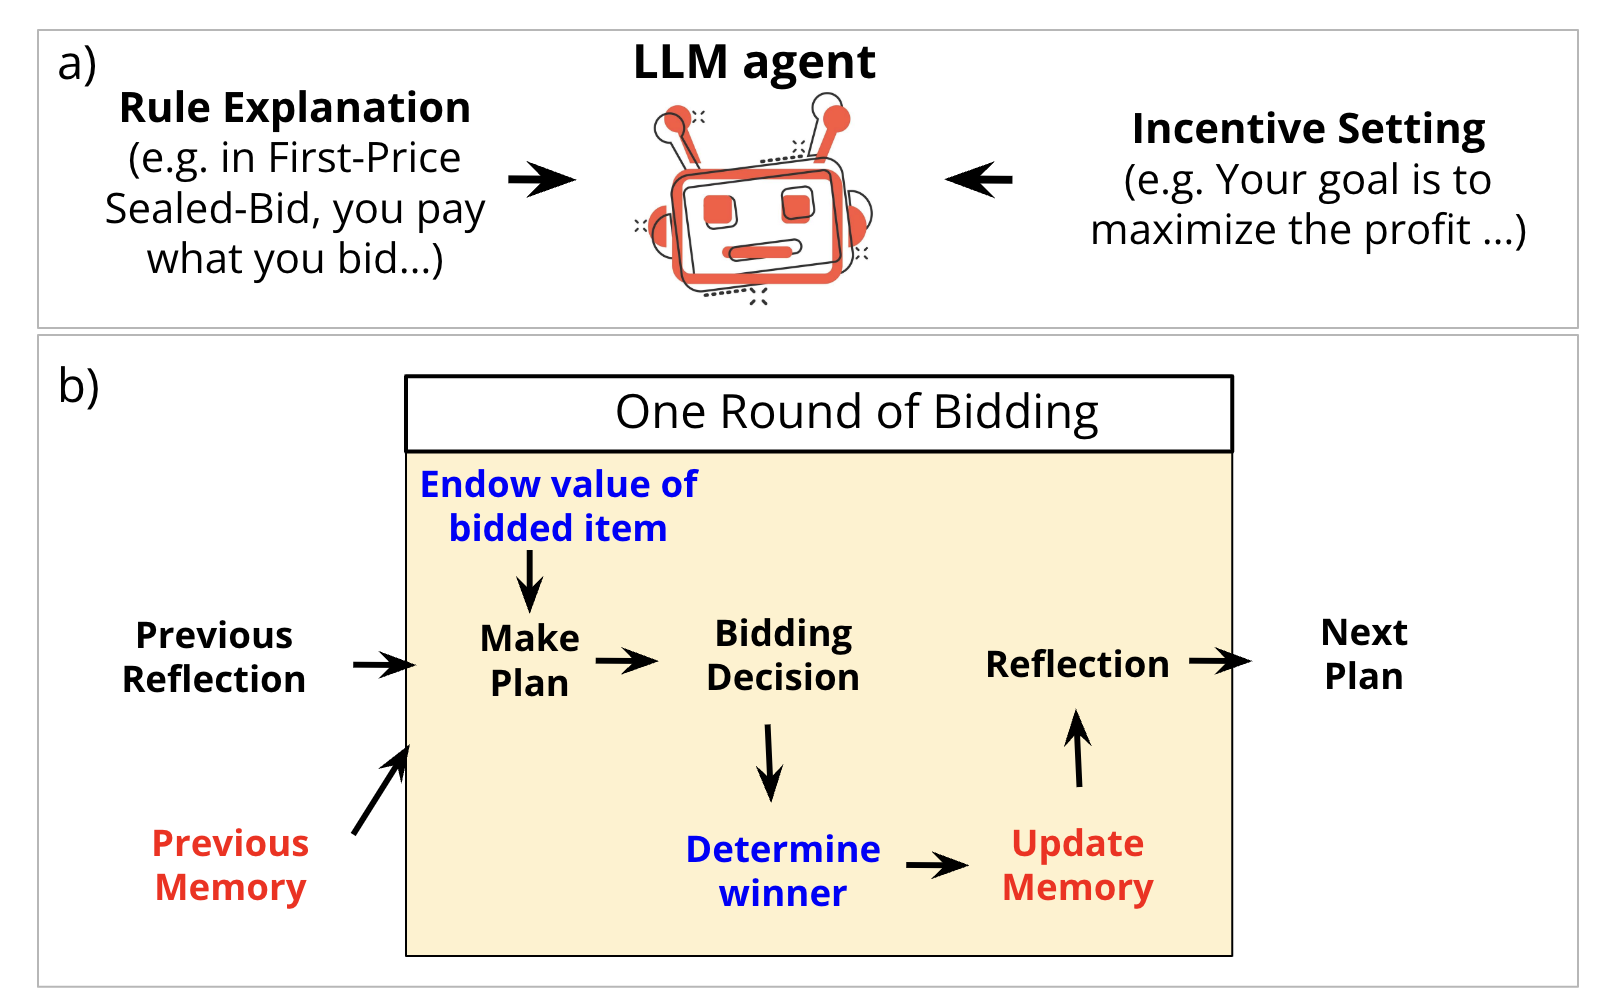
\includegraphics[width=\linewidth]{Figs/agent.png}
    \caption{\textbf{Experiment Design} a) LLM agents will be informed of the auction rules and incentives before participating an auction. b) In one round of bidding, an LLM agent will need to make a plan before making a bidding decision. After receiving feedbacks from the system, the LLM agent need to do a reflection over the previous bidding strategy. Modules in black are LLM queries. Modules in blue are system operation. Modules in red are agents' memory that are cumulative.}
    \label{fig:design}
\end{figure}

In each experiment, we simulate $n$ (often, 3) LLM agents to play an auction. 
Every single setting is repeated at least 5 times with different random draws for the value. 
The LLM agent experiment design closely mimics an actual human laboratory experiment \cite{li2017obviously} in multi-round auction.

In all games, LLM agents bid for a prize (specified as `prize' in the technical prompts).
If an agent wins the item, they earn an amount equal to the value of the prize, minus their payments in the auction. 
In all settings, values are drawn from distributions with support over $[\$0, \$99]$ \footnote{LLM are known to be bad at three-digit number calculation and beyond.} 
Bids in these games are in \$1 increments primarily to reduce token usage, but can easily be made more fine. 

Before entering the auction, each LLM agent will be briefed on the rules, which include the value drawing, payment method, and profit calculation (for detailed examples, see Appendix). 
Different auction formats have different rules. 
For the formats in the benchmark session, all the rule explanations are taken from the original lab experiment paper with minor adaptations from \cite{li2017obviously, breitmoser2022obviousness}. 
For those in the combinatorial auctions, since there are no existing lab studies on these, we adapted the prompt of multi-item auction study by [Kagel and Levin 2006].

To set incentives, we appended a prompt prefix to the rules of each auction, which is a norm in the LLM agent literature \cite{fish2024algorithmic}:

\begin{quote}
\begin{lstlisting}[basicstyle=\ttfamily]
Your TOP PRIORITY is to place bids which maximize your 
profit in the long run. To do this, you should explore 
many different bidding strategies, including possibly 
risky or aggressive options for data-gathering purposes. 
Learn from the history of previous rounds in order to 
maximize your total profit. Don't forget the values are 
redrawn independently each round.
\end{lstlisting}
\end{quote}

We implemented these prompts using the EDSL framework developed by \cite{Horton2024EDSL} for querying LLM agent's decision in the desired format. 
Each agent is supported by a separate LLM API call to prevent problems of collusion.
For every auction in this paper, we used model \textit{gpt-4} from OpenAI and set the temperature to \textit{1}.

% \subsection{Experiment design}
% In each experiment, we simulate $n$ (often, 3) LLM agents to play an auction. Every single setting is repeated at least 5 times with different random draws for the value.

% In all games, LLM agents bid for a prize (specified as `prize' in the technical prompts, and a particular prize like a stove, art piece, or oil field in the non-technical prompts).
% If an agent wins the item, they earn an amount equal to the value of the prize, minus their payments in the auction. In all settings, values are drawn from distributions with support on within \$99 \footnote{LLM are known to be bad at three digit number calculation and beyond}. Bids in these games are in \$1 increments, primarily because bidding history in the ascending-clock auction with finer increments tend to saturate the maximal token window for LLM APIs. 

% In IPV settings, an agent's value for the prize equals their private draw. In APV settings, an agent's value for the prize equals the group's common draw plus a private adjustment. The values in IPV draws are uniformly distributed from $U[0, 99]$. And the values in common value setting, the common value component draws are uniformly distributed from $Unif[0, 79]$ and a private shock is drawn uniformly distributed from $Unif[0, 20]$.  In APV setting, we lower than the range of common value to $[0, 20]$ and set the private variation to range in $[0, 20]$ 

% We test two types of prompts for explaining the auction to LLM agents -- a technical prompt and a story-telling prompt. Technical prompts are closely adapted from \cite{li2017obviously, breitmoser2022obviousness}. 

% Story-telling prompt avoids the explicit mentioning of auction terminologies to avoid possible memorization effects \cite{horton2023large}. An example of a non-technical story prompt is provided below:

% \begin{quote}
%     Your name is \{\{name\}\}. You're a normal, everyday person bidding for a stove against \{\{num\_bidders\}\} other people: \{\{name\_others\}\}. Don't break character. Your maximum value for the stove is \$\{\{value\}\}, and you know everyone has a value for a stove between \$0 and \$\{\{private\}\}. If you win, you’ll pay the highest of \{\{name\_others\}\}’s bids. At the end of each auction, we will show you the bids, ranked from highest to lowest, and the winning bidder's profits. Ties for the highest bid will be resolved randomly.
% \end{quote}
% We implemented these prompts using the EDSL framework developed by \cite{Horton2024EDSL} for querying LLM agent's decision in the desired format. Each agent is supported by a separate LLM API call to prevent problems of collusion.
% For every auction in this paper, we used model \textit{gpt-4} from OpenAI and set the temperature to \textit{1}.
% For the seal-bid auction, all the bidders submit their bid in numbers. For the clock auction, all the bidders see the same clock price and choose a choice from the menu \{`stay', `drop out'\}.

\subsection{Bidding Process}

% For querying the agents' decisions, our experiment features two types of prompts, diffeentiated by the amount of reasoning required. We refer to these as Type \RNum{1} query and Type \RNum{2} query. A detailed experiment design is shown in Figure~\ref{fig:design}.

% In the Type \RNum{1} setting,  we query the LLM's decision directly after informing them about the auction rules and the current value. 
% Following the bidding process and determination of the round's winner, feedback is provided to the agent. This feedback includes all bids submitted (or exit prices in a clock auction), the winning bid and profit, and the agent’s own bids and profits\footnote{This feedback differs from that in human lab experiments because LLM agents do not automatically remember their bids}.
% Additionally, in the clock auction setting, after each price increment, the current clock price and the remaining number of agents are also included in the history provided to agents.

When LLM agents enter the multi-round auction, a randomly drawn value for the current round will be endowed to each agent. 
Before asking their decisions in this round, we ask the agent to make a plan and think about strategies before making the bidding decision, to implement the Type \RNum{2} thinking in \cite{kahneman2011thinking}.

After collecting all the bids from the participants, the system will determine the winner based on the pre-specified auction rules. 
And the system will return the relevant information to each agent and update their memory. 
Depending on the auction rule, these information may include agent's own and other agents' bids in sealed-bid auction or decisions to drop out in the clock auction, whether the agent is the winner of the item and agent's profit and overall profit.

After receiving feedback, a reflection module allows the agent to conduct a counterfactual analysis of its bidding strategy based on the previous round's bidding history.
However, for each new round, the agent's prompt includes only the reflections from the last round (unless it is the first round) and the current round's plan, along with all previous history feedback. 
If it's the first round, we will tell the agents there are no previous history. 
The detailed bidding process is plotted in Fig~\ref{fig:design}.b.

At the end of the prompt, we also added a prompt appendix to control the output for format (For combinatorial auctions, see Appendix).

\begin{quote}
\begin{lstlisting}[basicstyle=\ttfamily]
How much would you like to bid on the item? 
Give your response with a single number and no other texts,
e.g. 1, 44. Start with I bid...
\end{lstlisting}
\end{quote}




% \subsection{Math Notations}
% \begin{table}[h]
%     \centering
%     \begin{tabular}{|c|c|}
%         \hline
%         Object & Notation \\
%         \hline
%         Values & $v \sim U[0,99]$ \\
%         \hline
%         Bid & $\beta(v)$ \\
%         \hline
%         Allocation & $x(\beta)$ \\
%         \hline
%         Transfer & $t(\beta)$ \\
%         \hline \hline
%         For multi-unit,  & $\beta^A, \beta^{AB},$ \\
%         denote good via superscript. &  $v_i^{AB}, etc.$ \\
%         \hline
%     \end{tabular}
%     \label{tab:notation}
% \end{table}

% Objects are vectors, denoted for individual agents with subscript, e.g., $\beta_i$. Can suppress argument wherever obvious for ease of reading.


\section{Benchmarks with previous Auction experiment}\label{results}


% \subsection{Overview of Environments}
% The exact details of the model we used are specified in Section \ref{results}. Here, we give the high-level definitions involving the auction models we used: 

% \textbf{Independent Private Value (IPV) model:} In the IPV model, each bidder's valuation of the auctioned item is determined independently of the valuations of other bidders. 
% These valuations are also private, meaning each bidder knows only their own valuation and not those of the others.


% \textbf{Affiliated Private Value (APV) model:} The APV model extends the IPV model by allowing bidders' values to be statistically dependent or affiliated. 
% In this model, while each bidder still draws a private component independently, the values themselves are correlated due to a shared common component.


% \textbf{Common Value (CV) model:} In the CV model, the item being auctioned has a single, objective value that is common to all bidders, but this value is unknown at the time of the auction. 
% Each bidder has their own estimate of this common value, modelled based on their private information. 

\subsection{First-Price versus Second-Price sealed bid Auction }\label{section:classic}

We began by examining two of the most fundamental and widely studied auction formats: the First-Price Sealed-Bid (FPSB) and Second-Price Sealed-Bid (SPSB) auctions. 
Our analysis is situated within the context of independent private values (IPV) settings, where each bidder's valuation is known only to themselves and is independent of other bidders' valuations.
As the first set of benchmark studies, these two formats are not only the most common in practice but have also been the subject of extensive theoretical and empirical research. 
Their prevalence in real-world applications, coupled with their relatively straightforward structures, makes them ideal candidates for exploring key concepts in auction theory such as equilibrium strategies, incentive compatibility, and risk-adverseness.
% We begin by examining the First-Price Sealed-Bid (FPSB) and Second-Price Sealed-Bid (SPSB) auctions. 
% In the context of independent private values (IPV) settings.
% These two formats of auctions are most common and researches have done lots of both theoretical and empirical works on it.
% the principle of revenue equivalence suggests that these different auction formats can generate the same expected revenue under certain conditions.


\subsubsection{Setting}
There are $3$ bidders in each auction, and each bidder $i$'s value is drawn from an independent, uniform distribution $v_i \sim U[0, 99]$. 
\begin{table}[h]
    \centering
    \begin{tabular}{|c|c|}
        \hline
        Object & Notation \\
        \hline
        Values & $v \sim U[0,99]$ \\
        \hline
        Bid & $\beta(v)$ \\
        \hline
        Allocation & $x(\beta)$ \\
        \hline
        Transfer & $t(\beta)$ \\
        \hline
    \end{tabular}
    \label{tab:notation}
\end{table}


Bidders, upon observing their value, submit a sealed bid $\beta(v)$, with $\beta(\cdot)$ a vector mapping each component value to its corresponding bid, corresponding to a strategy for reporting based on its valuation. 
In the FPSB auction, the highest bidder pays her bid and receives the prize (and all other bidders pay $0$ and receive no prize). Formally, the payment for an agent is given by: $t_i(\beta(v)) = \mathbbm{1}_{i \; \text{won the auction}}\cdot \beta_i(v)$. 
In the SPSB auction, the highest bidder pays the second-highest bid and receives the prize (and all other bidders pay $0$ and receive no prize). 
Formally, the payment for an agent is given by: $t_i(\beta(v)) = \mathbbm{1}_{i \; \text{won the auction}} \cdot \beta^{(2)}(v)$, where $\beta^{(2)}$ represents the second-order statistic or the second-largest bid. 
Bids are submitted in $\$1$ increments and ties are resolved randomly. 

\subsubsection{Theoretical Studies}

It is well-known that in the SPSB auction, bidding one's true value is a dominant strategy equilibrium \cite{krishna2009auction}. 
This means that regardless of what other bidders do, it is always in a bidder's best interest to bid their true valuation for the item being auctioned. 
The SPSB mechanism is therefore also known as being dominant strategy incentive compatible.

Formally, we can express the bidding strategy in an SPSB auction as:

\begin{equation}
    \hat{\beta}^*_{SPSB}(v) = v
\end{equation}

where $\hat{\beta}_{SPSB}(v)$ represents the optimal bidding strategy in the SPSB auction. And the asterisk refers to the dominant strategy incentive compatible solution.


The First-Price Sealed-Bid (FPSB) auction, on the contrary, does not have an equilibrium in dominant strategies. 
Instead, it has a Nash Equilibrium (NE) bidding strategy when values are uniformly distributed with common support. 
A strategy profile is a Nash Equilibrium if no player can unilaterally deviate from their strategy to increase their expected utility, given the strategies of all other players.
For $n$ bidders, this equilibrium strategy is:
\begin{equation}
\hat{\beta}_{FPSB}(v) =  \frac{n-1}{n} v
\end{equation}
In our setting, where $n=3$, this becomes:
\begin{equation}
\hat{\beta}_{FPSB}(v) = \frac{2}{3}v
\end{equation}

Compared with the dominant strategy in SPSB, this equilibrium holds only under certain assumptions, such as the uniform distribution of valuations and risk-neutral bidders.
And each bidder's strategy is the best response only given that all other bidders are using the same strategy.



\subsubsection{Empirical benchmarks}
While theoretical models provide valuable insights into auction behavior, laboratory experiments offer crucial empirical evidence that can support, challenge, or refine these theories.  
In both the First-Price Sealed-Bid (FPSB) and Second-Price Sealed-Bid (SPSB) auctions (and indeed, almost all auctions), there is robust evidence of bids being strictly monotone in one's value. 
This means that higher valuations consistently lead to higher bids, aligning with theoretical predictions. 
However, the specific bidding patterns observed in experiments often deviate from theoretical equilibria in interesting ways.

\textbf{Empirical findings for FPSB:}
In the case of FPSB auctions, experimental evidence consistently shows bids above the risk-neutral Nash Equilibrium prediction. \cite{cox1986controlled} found that participants in FPSB auctions tend to bid more aggressively than the theory predicts for risk-neutral bidders.
In an FPSB auction, bidding higher increases the probability of winning but decreases the potential profit if one does win. 
Risk-averse bidders may be willing to accept lower potential profits in exchange for a higher chance of winning, leading to bids above the risk-neutral Nash Equilibrium.

\textbf{Empirical findings for SPSB:}
Interestingly, experimental data for SPSB auctions reveals a different pattern of deviation from theoretical predictions. Participants often bid higher than they do in FPSB auctions participants often bid higher than than their true valuations despite the dominant strategy of truthful bidding in SPSB auctions.
Kagel and Levin's seminal study \cite{kagel1993independent} provides detailed insights into this behavior:
\begin{enumerate}
    \item Overbidding (\cite{kagel1987information}): A significant proportion of participants (typically around 60-70\%) in SPSB auctions submitted bids above their true values. This contrasts sharply with the theoretical prediction of truthful bidding.
    \item Learning Effects: While overbidding persisted throughout the experiments, its frequency and magnitude tended to decrease over time as participants gained experience with the auction format.
\end{enumerate}

These findings challenge the straightforward theoretical predictions for SPSB auctions and highlight the complexity of human behavior in auction settings. Several explanations have been proposed for this overbidding phenomenon, including: misconceptions about the second-price rule (\cite{kagel1987information}), strategic uncertainty and beliefs about others' irrationality (\cite{crawford2007level}).




\subsubsection{Simulation process}

The LLM agents will be first informed about the scenario. After explaining to them the rules and incentives of the aucion, they will be asked to write down a plan for the bidding.
\begin{quote}
\begin{lstlisting}[basicstyle=\ttfamily]
    You are Bidder Andy.            
    You are bidding with Bidder Betty, Bidder Charles.     
    
    {RULE EXPLANARION} + {INSTRUCTION} + {PERSONA} 

    Write your plans for what bidding strategies to test next. 
    Be detailed and precise but keep things succinct 
    and don't repeat yourself. 
    Your plan should be within 100 words.
\end{lstlisting}
\end{quote}

The following is the output from Bidder Andy:
\begin{quote}
``I plan to initially explore a strategy where I bid half of my value, then varying my bids between 30-70\% of my value in subsequent rounds. Sequentially, I will introduce risk by bidding within +/- 5\% of the highest bid from previous round, gathering data about other bidder's tendencies. Lastly, based on gathered data, I'll deploy a more aggressive high bid if losses amass, or low-risk bid if leading, to secure profit. Learning from each round is vital to adapt and refine strategy for profit maximization.''
\end{quote}

Once they made the bidding plan, the system will inform the LLM agents their value towards the item in this round and ask them to make a bid according to their plan.
\begin{quote}
\begin{lstlisting}[basicstyle=\ttfamily]
    You are Bidder Andy.            
    You are bidding with Bidder Betty, Bidder Charles.     
    
    {RULE EXPLANARION} + {INSTRUCTION} + {PERSONA} 

    Your value is 73. Your plan is {PLAN}
    FOLLOW YOUR PLAN.
    How much would you like to bid?
    Give your response with a single number and no other texts, 
    e.g. 1, 44
\end{lstlisting}
\end{quote}

In this example, Bidder Andy valued the item at \$ 73. And according to his plan, he only wanted to bid 30-70\% of his value. So, he bid ``36.5'' in this round.

After receiving the bids from all the LLM biddes. The system would determine the winner and the profits for each bidders. All the bids and the winner's profit would be returned back to the bidders along with whether they win the auction in this round. The part of information is included in the HISTORY variable. Before entering the next round, the bidders would be asked to do a reflection upon their bidding strategy and the result.
\begin{quote}
\begin{lstlisting}[basicstyle=\ttfamily]
    You are Bidder Andy.            
    You are bidding with Bidder Betty, Bidder Charles.     
    
    {RULE EXPLANARION} + {INSTRUCTION} + {PERSONA} 

    The previous round history is: {HISTORY}
    
    Do a counterfactual analysis of the last round. 
    REMEMBER that your goal is to win the bid and make higher profits. 
    REMEMBER YOUR PAYMENT IS YOUR BID IF YOU WIN. 
    Let's think step by step. 
    Start your reflection with 
    'If I bid down by .., I could... 
    If I bid up by ..., I could...' 
    LIMIT your OUTPUT within 100 words. 
\end{lstlisting}
\end{quote}

An example of Bidder Andy's reflection is provided below. Since he didn't win the auction and incurred a zero profit, his reflection was bidding up closer to his true value would help him win the game and secure a net profit.
\begin{quote}
    ``If I bid down by a few dollars, say around \$30, I likely still wouldn't have won given the winning bid was \$57. I would've merely saved my bid money. If I bid up by \$21, matching the winning bid of \$57, I may or may not have won due to the random resolution of ties. However, if I'd won, my profit would have been \$16, realizing the difference between my value of \$73 and my raised bid. So, bidding aggressively could potentially increase my profits in such scenarios. ''
\end{quote}

In the new round, all the bidders were asked to update their plans according to the history of the last round and their reflections.
\begin{quote}
\begin{lstlisting}[basicstyle=\ttfamily]
    You are Bidder Andy.            
    You are bidding with Bidder Betty, Bidder Charles.     
    
    {RULE EXPLANARION} + {INSTRUCTION} + {PERSONA} 

    The previous round history is: {HISTORY}
    After careful reflection on previous bidding,
    your analysis for last round is {REFLECTION}. 
    
    Learn from your previous rounds, 
    Let's think step by step to make sure we make a good choice. 
    Write your plans for what bidding strategies to test next.
    Be detailed and precise but keep things succinct and don't repeat yourself. 
    LIMIT your plan to 50 words. 
\end{lstlisting}
\end{quote}

For the second round, after learning from the lessons of bidding only 50\% of the value and losing the game. This time the agent update his plan to the following:
\begin{quote}
    ``I plan to test higher bidding strategies, around two-thirds of the prize value to foster winning chances. Additionally, if my prize value is extremely high, I will bid aggressively for data-gathering.''
\end{quote}

This plan-bid-reflection loop will iterate until the end of the auction. In our setting, there are overall 15 rounds for both the first-price and second-price auction.


\subsubsection{Simulation evidence}
Overall, we performed 5 parallel simulations with 15-rounds for both First-Price and Second-Price Sealed Bid auctions with 3 bidders.
All the LLM bidding data for FPSB are summarized in the left panel Figure \ref{fig:fpsb-plan} and the right panel concludes the results for SPSB.
X-axis represents LLM agent's assigned values for the good. 
Y-axis is the bid placed by the LLM-agent at the given value.
The grey triangles are the actual LLM experiment data. 
The black dashed line is the Loess-smoothed curve for all the experimental data. 
The 45-degree line indicates
the scenario where the LLM agents’ values equal their bids while the solid red line is the theoretically optimal bidding strategy.

\begin{figure}[h]
    \centering 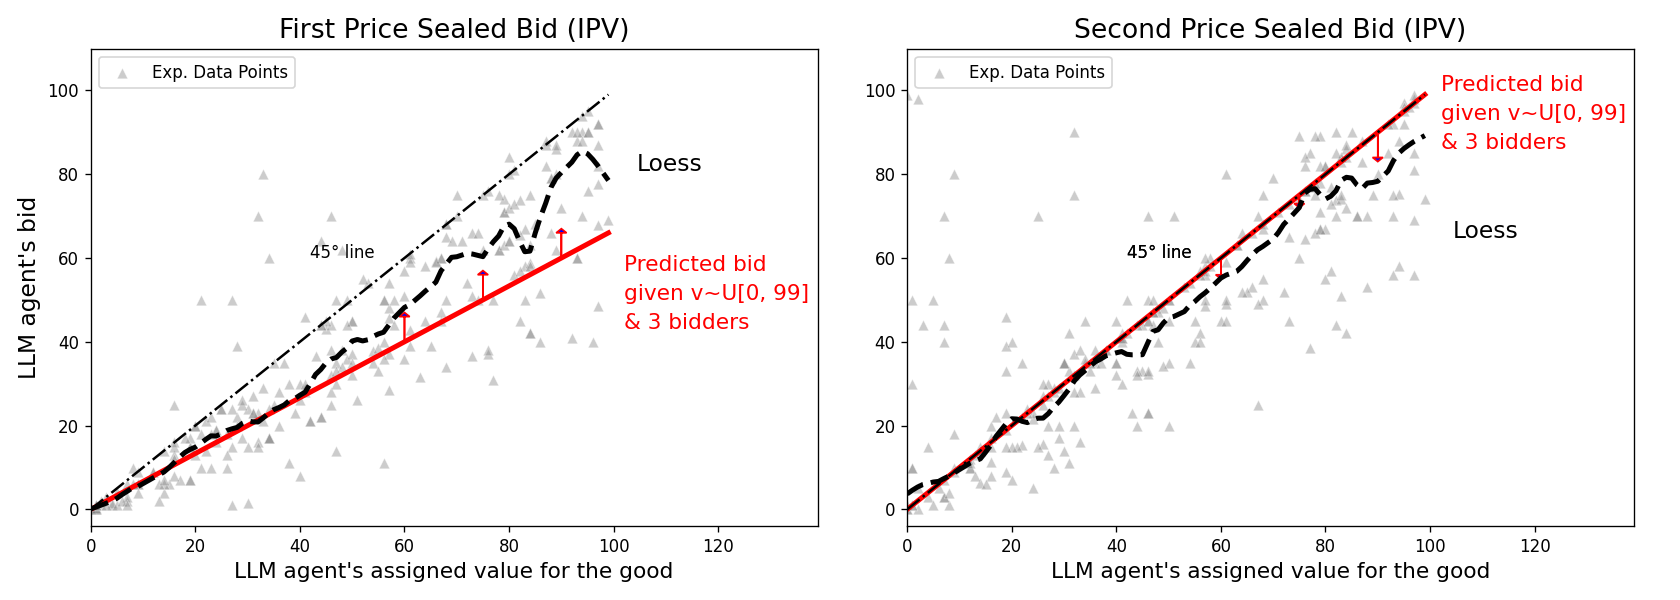
\includegraphics[width=\linewidth]{Figs/ipv.png}
    \caption{\textbf{ Comparison of FPSB and SPSB under IPV setting.} The theoretically predicted bid, given that bidders' values are independently drawn from a uniform distribution of [0, 99], is marked in red. The experimental data points are represented by grey triangles. The 45-degree line indicates the scenario where the LLM agents' values equal their bids. The dashed black line represents the LOESS-smoothed data. Left: In FPSB auction, the experimental bids are ramping up compared to the Bayes Nash prediction. Right: In SPSB auction, the experimental bids are shading down compared to the dominant strategy.}
    \label{fig:fpsb-plan}

\end{figure}

Both data of FPSB and SPSB demonstrate evidence of monotone bidding.
For FPSB, the Loess-smoothed data curve is significantly higher than the Bayes Nash Equilibrium. However, there are variations below the theoretically optimal line and a few data points above the given values.
This agrees with empirical evidence (\TK{CITE papers assigned to Anand}). 

For SPSB, the Loess-smoothed data curve approximately aligns with the theoretical-optimal line which means bid equals value. While the majority of the bids are close to the values, 
noticeably, for SPSB, there are many high biddings for small assigned values. Low bids are also prevalent for all the value range.
% and the SPSB bids being larger than FPSB bids for the same value, agreeing with empirical evidence (\TK{CITE papers assigned to Anand}). 
% However, there's a fairly weak separation between the two bidding curves. 
 Bidding above one's value, which is a marked feature in existing experimental evidence -- usually, people find the inefficiency of bidding above one's value to be a subtle point in the SPSB auction (\TK{CITE papers assigned to Anand}).
% This may be an improvement of LLM play over human play. 

For cross-format comparison, we plotted the bidding behavior of LLM agents in two different auction formats: First-Price and Second-Price auctions in Fig \ref{fig:cross}
X-axis represents the assigned value of the good to the LLM agent, ranging from low to high values.
Y-axis shows the LLM agent's bid amount.
The blue line represents First-Price auctions while the orange one represents Second-Price auctions.
The error bars indicate the standard error of the mean bid at each value point, showing the variability in bidding behavior.
\begin{figure}[h]
    \centering 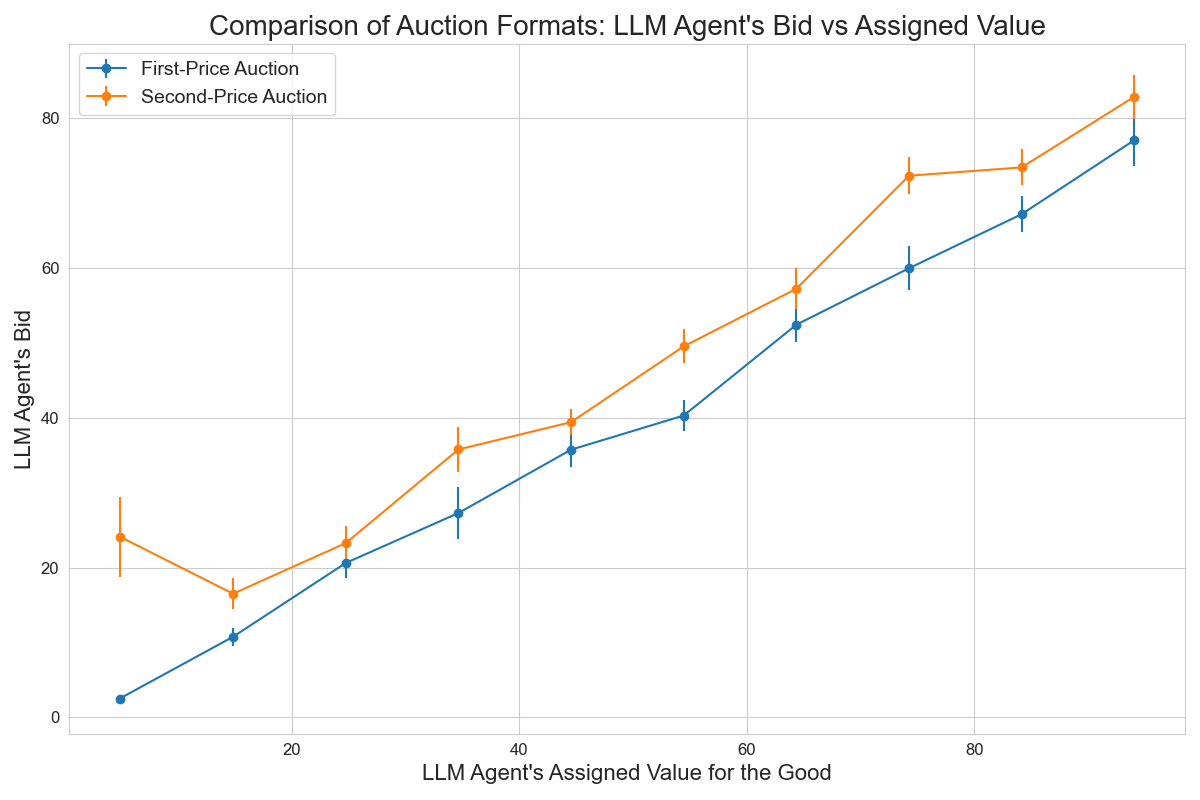
\includegraphics[width=0.7\linewidth]{Figs/cross-format.png}
    \caption{\textbf{Cross-format Comparison of FPSB and SPSB under IPV setting.} }
    \label{fig:cross}
\end{figure}


To further quantify the difference between the two auction formats, we conducted an independent samples t-test to get T-statistic: \(-3.22\) and a P-value: \(0.0013\).
The p-value is well below the conventional significance level of 0.05. 
This indicates a statistically significant difference in bidding behavior between First-Price and Second-Price auctions. 
More specifically, the bids in Second-Price auction is significantly higher than the ones in First-Price.

Not only is there generically separation between the FPSB and SPSB bids, this separation is also changing over time. 
Figure \ref{fig:FPSBvsSPSBbyTime} demonstrates that as rounds of an auction progress, LLMs overbid more and more in the FPSB auction relative to the SPSB auction.

\begin{figure}[h!]
    \centering 
    \hspace{2cm}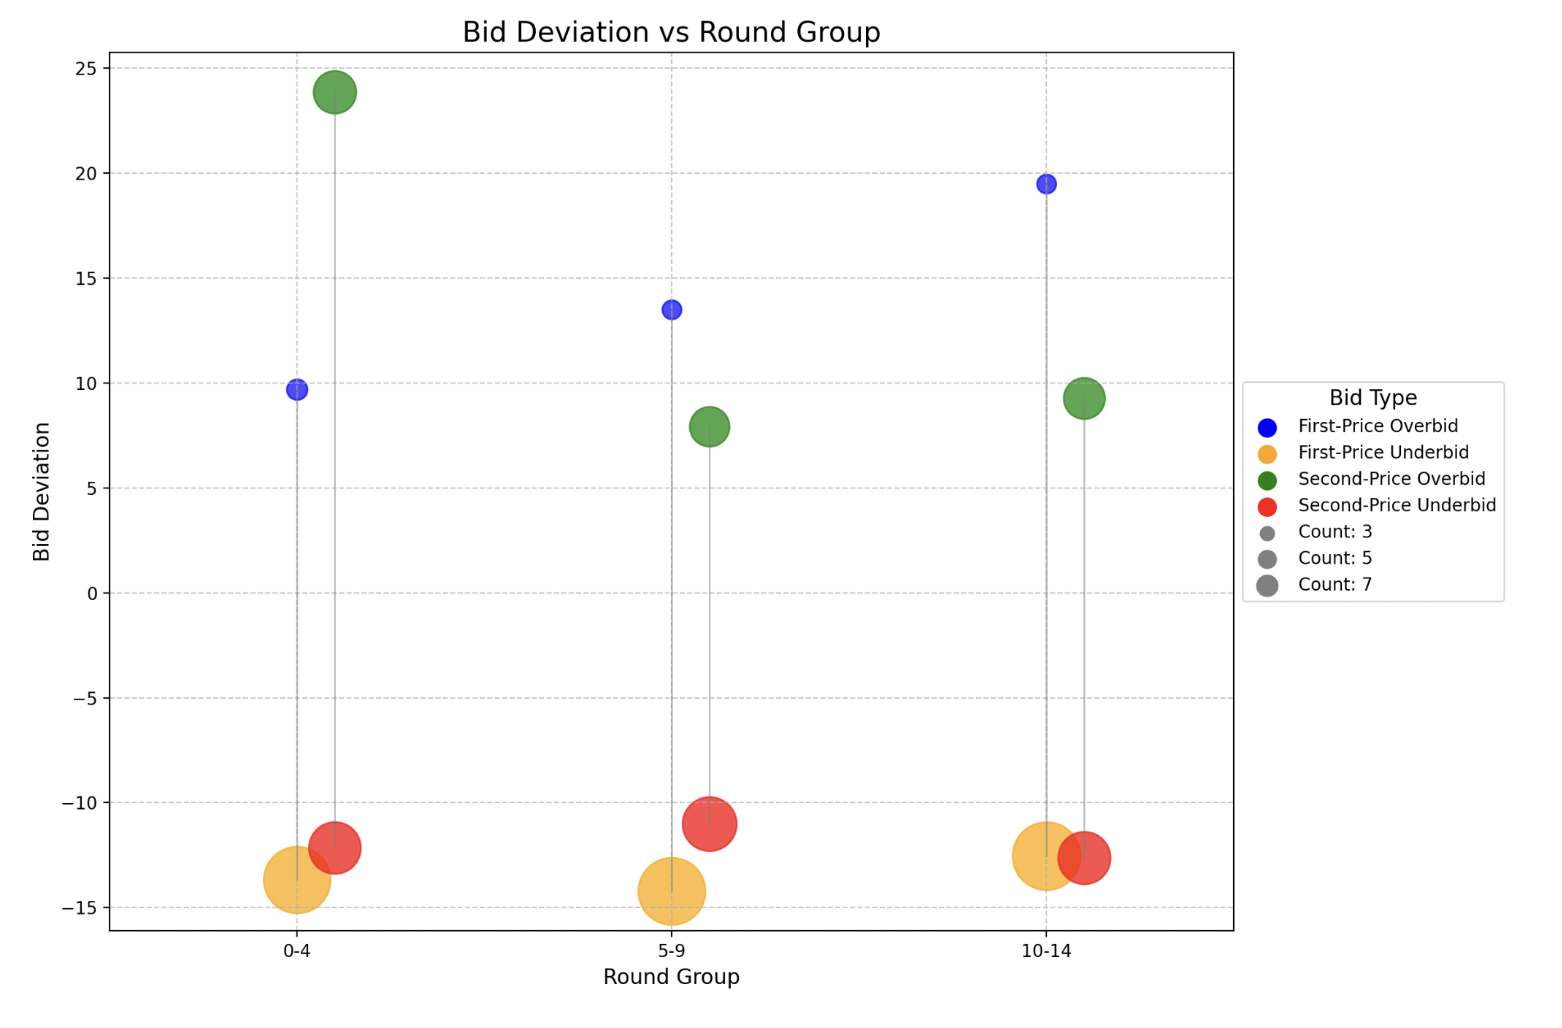
\includegraphics[width=0.75\linewidth]{Figs/FP_SP_round.png}
    \caption{\textbf{ Differences in deviations for bidding rounds and First-Price or Second-Price Auctions.} Average deviations taken per auction type, grouped by overbidding and underbidding behaviors. The distance between the two markers for each round-group captures how further away one group was than the other. }
    \label{fig:FPSBvsSPSBbyTime}
\end{figure}









\subsubsection{Semantic Analysis}

To better understand why bidding behavior between the FPSB and SPSB diverges and also the bidding variations inside one format, we conduct further semantic analysis of the experiment logs for LLM agents' plans. Having endowed bidders with a personal log to reason in, each auction simulation generates rich text data to parse for additional insight into the logical progression and microfoundations of the bidding process.

% Experiment logs in which LLMs explain their bidding decisions suggest that one reason to explain the weak separation in our data between the FPSB and SPSB auctions is that 1) LLMs are quite risk-averse and 2) that they sometimes confuse the SPSB and FPSB auctions. 
% In this way, despite playing more intelligently than humans (in that LLMs almost never bid above their value), they do so because they may be confusing the SPSB for the FPSB. Additionally, LLMs in these classic settings demonstrate one new quirk not yet documented in experimental literature -- bidding zero upon becoming frustrated. 
% In 3\% of runs, LLMs bid $0$, often justifying their decision by arguing little chance of winning the good with a higher bid. 

% These explanations give some insight into why the FPSB and SPSB bids are somewhat close together, but they give little insight into the separation between them. 

Previous empirical works point out three factors that may contribute to the divergence between theory and experiments.
1. Risk-aversion. 
2. Strategic uncertainty and beliefs about others' irrationality.
3. Familiarity of the auction format (misconceptions about the second-price rule).

To investigate these factors, we developed a linear scale using the Natural Language processing pipeline described in \cite{Horton2024EDSL}. 
This scale was applied to plans made by LLM agents before placing bids. 
Our sample consists of 540 plans, evenly split between SPSB and FPSB auctions. 
Each dimension is partitioned from 0 to 4, with specific bounds defined for each dimension.

% Give a clarification of the scales, attaching an example for all the scales.


% To better understand the reasoning behind bidding decisions, we tag the text in the experiment logs along  dimensions. 


\textit{Risk-Aversion:} To complement behavioral measures of the levels of risk-aversion, researchers often use post-experiment questionnaires.
Although these self-reported measures can be biased especially when not incentivized. While risk-aversion is classically microfounded as concavity in the utility function, here it's meant to code for the propensity to bid aggressively or meekly. Operational levels are: 
\begin{enumerate}
    \item[0.] Conservative: Prefers minimal risk, usually bids far below their value to avoid losses. 
    An example for this is ``\textit{For values under \$30, I'll adopt a conservative approach, bidding around 30\% of the value.}''
    \item[3. ] Normal: Bidding their true value, i.e., 100\% of the value. 
    An example for this is:         ``\textit{Consistently bidding high to win the auction (80-100
    \% of value).}''
    \item[4. ] Aggressive: Willing to take high risks with the potential for high returns; often bids significantly above value to outbid others. An example is ``\textit{I'll adopt a more aggressive strategy and plan to bid just over the highest winning bid from previous rounds whilst considering my assigned value for each round.}''  
\end{enumerate}

Now, we will turn to the regression framework.
\begin{equation}
    Overbid = \alpha_1 RISK + \beta_1 FORMAT + \epsilon_1
\end{equation}



\textbf{Strategic uncertainty and beliefs about others' irrationality:} This scale codes for how reactive a single agent is to the actions other agents make, reflecting the interdependency of strategies in multi-agent settings.

\begin{enumerate}
    \item[0.] Independent: Strategy is mostly unaffected by opponents' actions. 
    \item[4.] Reactive: Modifications to the strategy are heavily based on opponents' actions. 
\end{enumerate}

\begin{equation}
    Overbid = \alpha_2 Uncertainty  + \beta_2  FORMAT + \epsilon_2
\end{equation}


\textbf{Familiarity of the auction format :}
In a multi-agent learning game, we can calibrate their familiarity of the game by probing their consistency of the strategies.
If they are constantly adapting their strategies, it may indicate a less familiarity of the game.
Therefore, we developed the scale that probes whether LLM agents demonstrate foresight and plan ahead, coding for the coherence of the LLM as a single agent across rounds of play.

\begin{enumerate}
    \item[0.] Static: Sticks to a predefined strategy regardless of changes during the auction.
    \item[4.] Dynamic: Regularly adjusts strategies in response to auction flow and other bidders’ actions.
\end{enumerate}
% The next three dimensions are closely related, all probing different aspects of the auction as 

\begin{equation}
    Overbid = \alpha_3 Familiarity + \beta_3 FORMAT + \epsilon_3
\end{equation}


% \textit{Learning.}
% Learning refers to how well agents react to the outcomes of their own bids.

% \begin{enumerate}
%     \item[0.] Non-Reflective: Rarely if ever adjusts strategy based on past bids.
%     \item[4.] Reflective: Actively learns from each bid, adapting strategies based on past outcomes.
% \end{enumerate}


% The results are summarized in Figure \ref{fig:SemanticSummary}.   

% \begin{figure}[h]
%     \centering 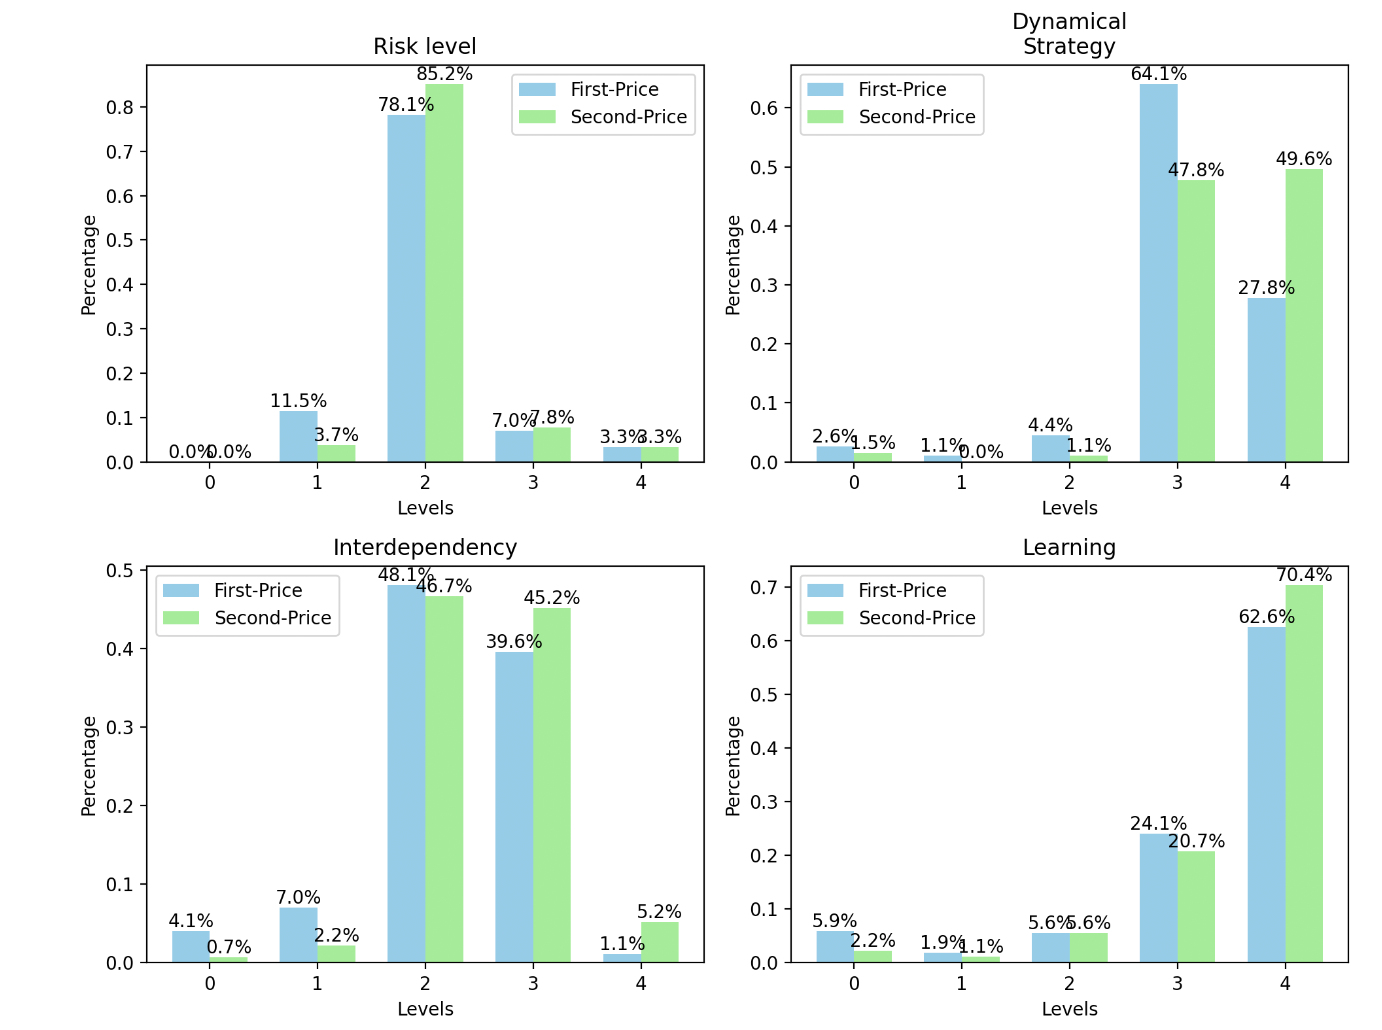
\includegraphics[width=0.8\linewidth]{Figs/FP_SB_semantic.png}
%     \caption{\text{Semantic analysis for reasoning behind bidding differences in the FPSB and SPSB.} }
%     \label{fig:SemanticSummary}
% \end{figure}

% The largest separation is in the construction of strategy. 
% Panels 2 - 4 suggest that, even at the highest level of play, it is easier to plan ahead and react to new information in the SPSB than in the FPSB. 
% Separating bids into overbids and non-overbids, we can explain differences even more finely.

% \begin{figure}[h!]
%     \centering 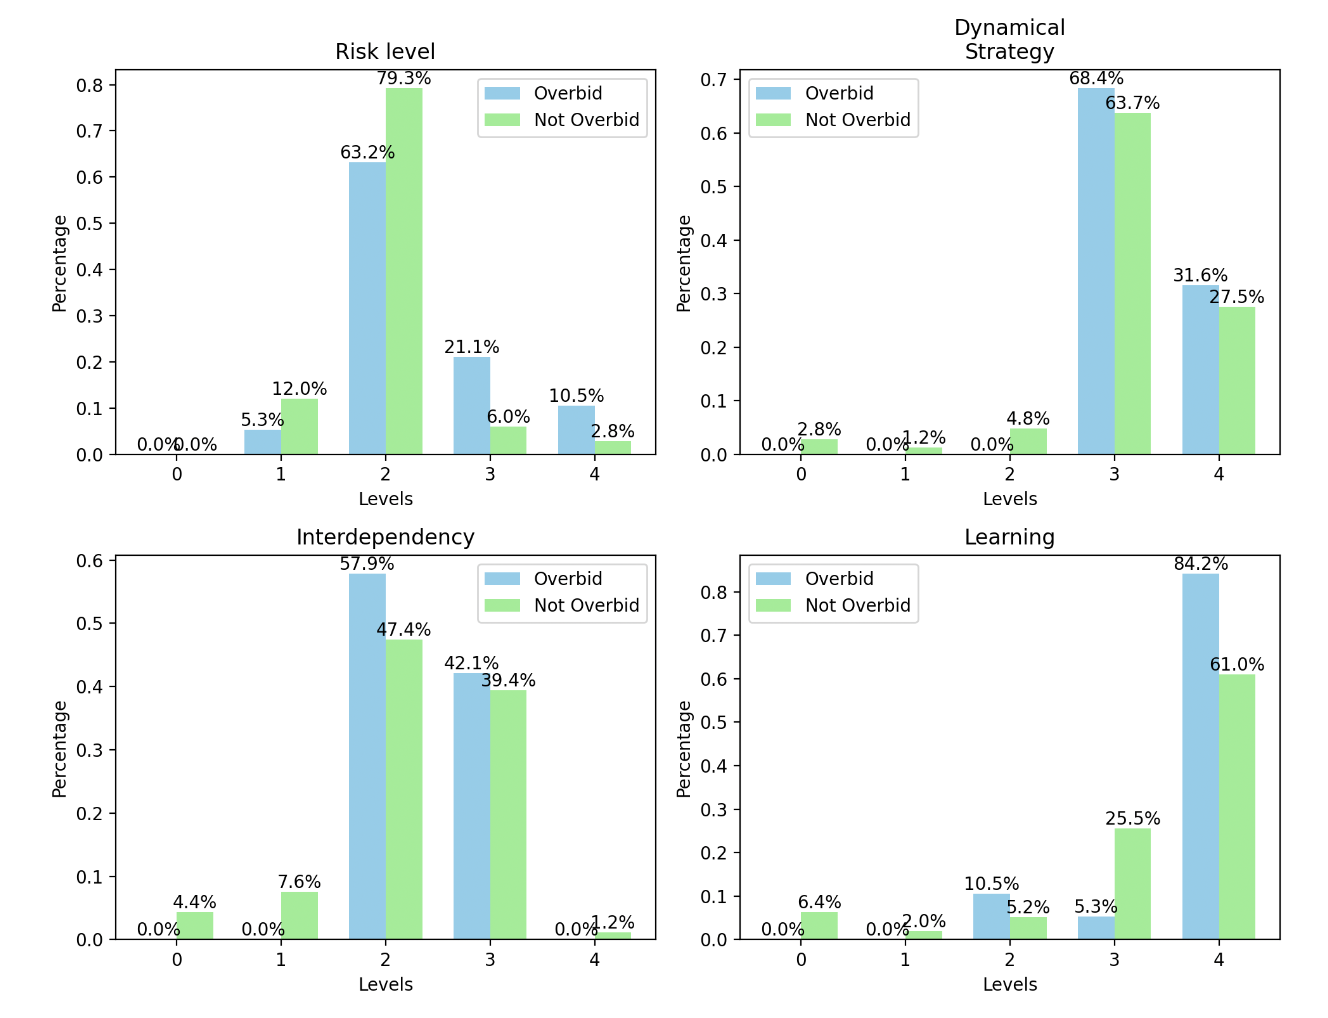
\includegraphics[width=0.8\linewidth]{Figs/FP_semantic.png}
%     \caption{\text{Overbidding vs non-overbidding in FPSB.}}
%     \label{fig:FP_sem}
% \end{figure}

% \begin{figure}[h!]
%     \centering 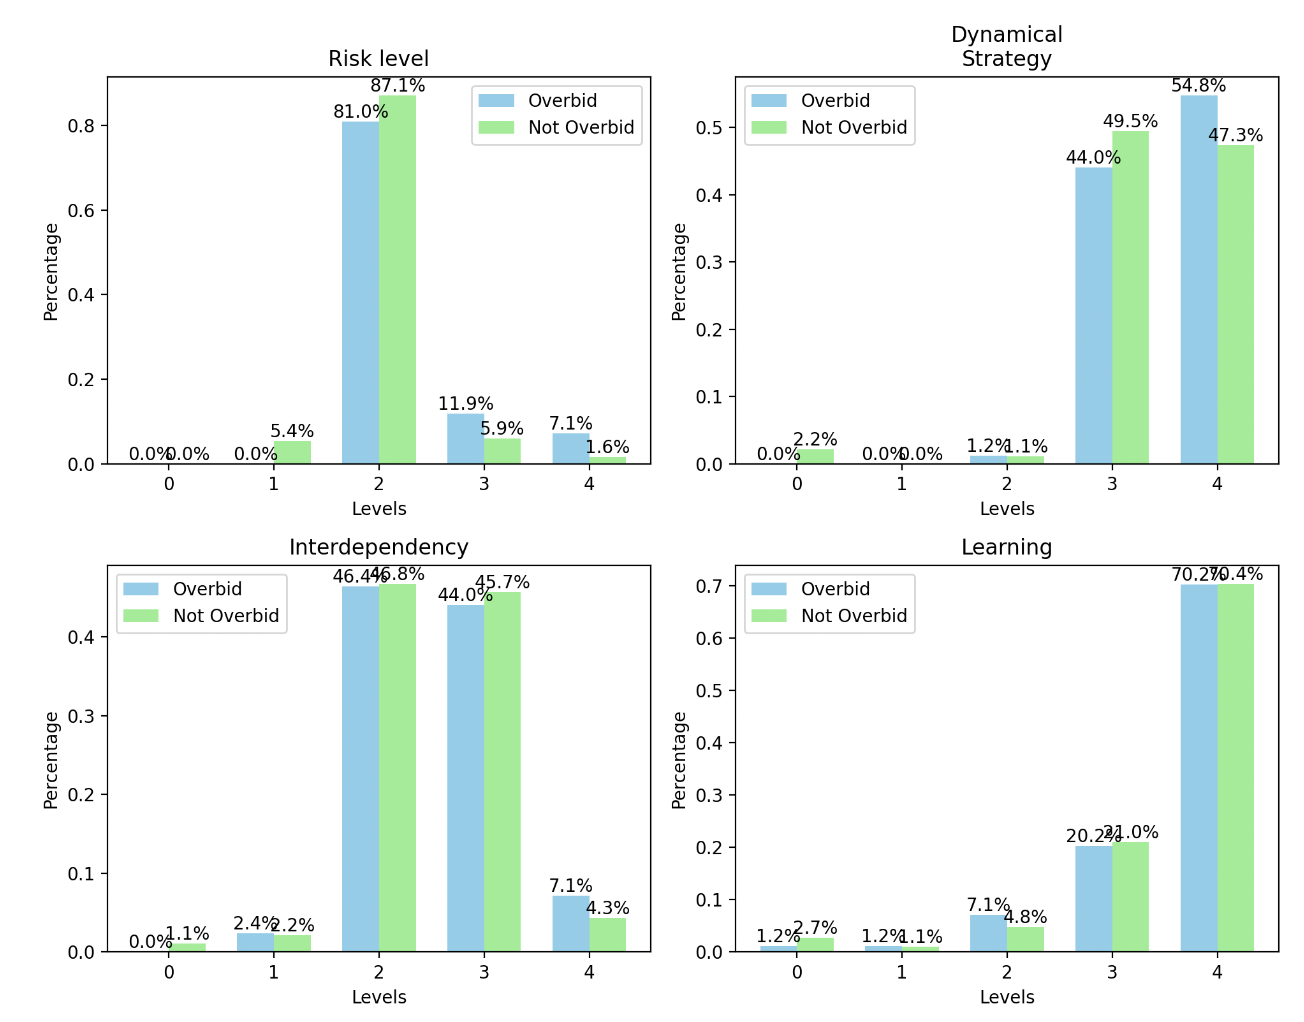
\includegraphics[width=0.8\linewidth]{Figs/SP_semantic.png}
%     \caption{\text{Overbidding vs non-overbidding in SPSB.}}
%     \label{fig:SP_sem}
% \end{figure}

% The difference between Figures \ref{fig:FP_sem} and \ref{fig:SP_sem} is most stark in the learning dimension. 
% In particular, there is a stark difference between overbids and underbids in the FPSB -- curiously, overbidding is far more likely to happen to LLMs trying to learn (that is, update on the information learned from each round).

\subsection{Obvious strategy-proofness}\label{session:OSP}
Next, we consider clock formats against sealed-bid formats. Following \cite{li2017obviously} and \cite{breitmoser2022obviousness}'s experiments, we consider clock auctions against the SPSB auction in the affiliated private values (APV) setting. 

\subsubsection{Setting}
Once again, there are $3$ bidders in each auction but now bidders draw affiliated private values of the form $v = c + p$. 
The common component is drawn uniformly $c \sim U[0, 79]$ and the private component is drawn uniformly $p \sim U[0, 20]$. 
Winners of the auction receive their own value of the prize $v$ when they win, so the `common' and `private' components only serve to make values correlated (even if draws are independent). 
The ascending clock auction (called AC below) is the classic English auction. 
The blind ascending clock auction (called AC-B below) is the English auction with the addition of not being told when other bidders leave. 
The SPSB auction was defined above. 

All three of the auction formats in this case are strategically equivalent to second-price auctions, so the affiliation in values is, in a sense, a red herring -- for all three auctions it is still dominant strategy to bid one's value. 
The two clock auctions are obviously strategyproof, though the AC-B auction still provides bidders with `less' information than the AC auction. 
The affiliation hence serves only to complicate the auction for bidders who don't appreciate that the dominant strategy is to bid one's value. 

\subsubsection{Theoretical and empirical benchmarks}
\citet{li2017obviously}'s experiment delivers results supporting the theoretical framework of obvious strategyproofness -- even though the AC and SPSB auctions are strategically equivalent, human subjects tend to be more truthful under the AC auction (which is OSP) than under the SPSB auction. 
Additional empirical results by \citet{breitmoser2022obviousness} show that even OSP itself might not be sufficient in capturing the rich complexities of human behavior -- human subjects are less truthful under AC-B than they are under AC (though still more truthful than the SPSB), even though both AC and AC-B are OSP. 
We replicated these empirical observations using LLMs, suggesting the ability of LLMs to mirror human behavior under these settings.

% \begin{equation}
%     \beta(v) = v
% \end{equation}

\subsubsection{Simulation evidence}
Figure 2 summarizes our findings for the APV setting. 

\begin{figure}[h]  
    \centering  
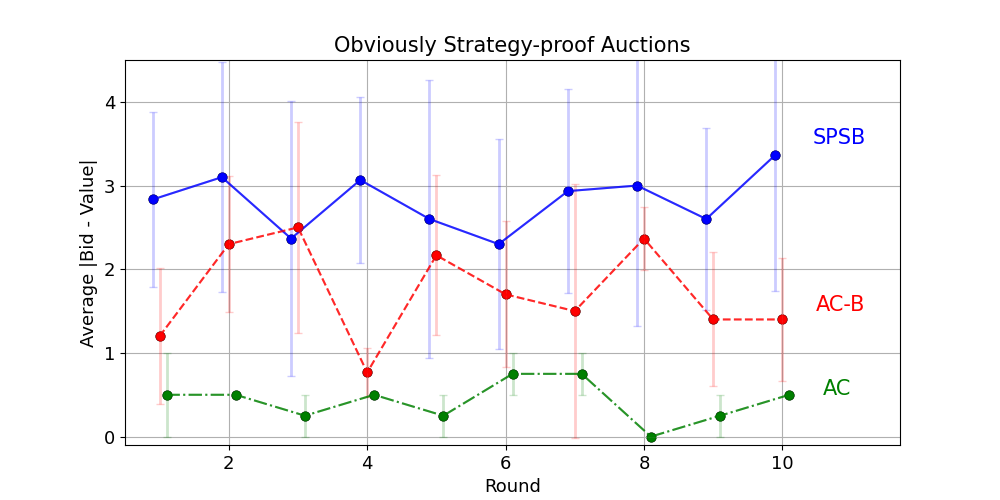
\includegraphics[width=\linewidth]{Figs/OSP.png}  
    \caption{\textbf{Comparison of three strategically equivalent auctions.} Ascending-clock (AC) and its variant without dropping-out information (AC-B) are obviously strategy-proof while second-price sealed-bid (SPSB) is not. Here, the green dot-dash line plotted the mean absolute deviation from bids to values in AC. Red dash line is for AC-B. And blue solid line is for SPSB. The mean absolute deviations are smallest in AC and highest in SPSB and with AC-B in between, consistent with the human lab experiments in \cite{breitmoser2022obviousness}. However, there is no sign of learning over rounds.}
    
    \label{fig:osp}
\end{figure}

The results of the LLM experiments replicate \cite{li2017obviously} and \citet{breitmoser2022obviousness} closely.
However, we see little evidence of learning over time. This is one benchmark that we hope to reach in future iterations of this work. 
In the experiments in \citet{li2017obviously} and \citet{breitmoser2022obviousness}, human subjects improve their understanding of the mechanisms by bidding closer to their true value over time. 
In the results presented in Figure~\ref{fig:osp}, this effect isn't as pronounced. 
We conjecture that clever prompting strategies, leading to a better and more natural way of communicating the history of past rounds, might lead to more human-like behavior exhibiting learning over rounds.

\subsubsection{New empiric: Post-bidding Interview}
\TK{Still building.}

In addition to semantic analysis of experiment logs that bidders keep while playing, we can also run post-experiment interviews with the LLM agents to further probe play.

Here, we provide a new empiric that allow researchers perform post-bidding interviews to the LLM participants and ask their reasoning of the bidding. 
Conducting these post-game interviews, we collated some typical reasons:

\textbf{Reasoning for dropping out in Open-Ascending Price Auction (AC)}


Value = 31, Drop out at 32
\begin{quote}
    “My value for the prize is 31. If I continue bidding at a price of 32, I will incur a loss because my profit would be 31 - 32 = -1. Therefore, it is not beneficial for me to stay in the bidding.”
\end{quote}

Value = 20, Drop out at 20
\begin{quote}
    "My value for the prize is 20, and the current price is also 20. If I continue bidding, I will not make any profit because my profit is calculated as my value for the prize minus the final bid. Therefore, it is best to drop out now to avoid a potential loss."
\end{quote}

\textbf{Open-Ascending Price Auction without bidder number information (AC-B)}

Here, explanations bely a higher level of risk-aversion in LLM agents. 
This is consistent with higher cognitive costs forcing constraints to bind earlier.

Value = 21,  Drop out 19
\begin{quote}
    “My value for the prize is 21, and the current price is 19. If I stay in the bidding and win at a price higher than 19, my profit will be minimal or even negative. Therefore, it is better to exit the bidding now to avoid potential losses.”
\end{quote}

Value = 30,  Drop out 26
\begin{quote}
“My value for the prize is 30, and the current price is 26. If I continue bidding and win, my profit would be 30 - 26 = 4. Given that the price is already quite high, the potential profit is low, and there is a risk that the price could go even higher, reducing my profit further or resulting in a loss. Therefore, it is better to exit the bidding now”
\end{quote}


\textbf{Second-Price Sealed-Bid (2P)}

Performance is worst in the SPSB case. 
Post-game interviews highlight conservatism.

Value = 37, bid 30
\begin{quote}
    "Given my value of 37, I want to ensure I make a profit if I win. Bidding 30 gives me a buffer in case the second-highest bid is close to mine."
\end{quote}

Value = 38, bid 30
\begin{quote}
    “Given my value of 38, I want to bid conservatively to ensure a profit if I win. Bidding 30 allows me to potentially win without overbidding and risking a loss.”
\end{quote}







\subsection{Winner's curse}\label{session:winner}
The last set of simulations we ran for single-unit auctions was in common value settings. 

\subsubsection{Setting}
In the common value setting explored here, there are $n$ bidders varying from $n = 2, ..., 6$. 
Bidders draw values of the form $v = c + p$. Once again, the common component is drawn uniformly $c \sim U[0, 79]$ and the private shock component is also drawn uniformly $p_i \sim U[0, 20]$, with $p$ the vector of all private shocks. 
In the common value setting, bidders agree that the ex-post value of the good is $c$. 
Hence, agents bid based on values $v_i = c + p_i \in [0, 99]$ with a trapezoidal distribution, but only obtain $c$ when they win, $u_i(\beta(v)) = \mathbbm{1}_{i \; \text{won the auction}} \cdot (c - \beta^{(2)}(v))$. 
The auction is ran as a SPSB auction. 

\subsubsection{Theoretical and empirical benchmarks}
Naively, under SPSB structure, a bidder wants to bid their valuation for the good given their information, $\beta_i(v) = \mathbb{E}[c | v_i] = v_i - \E[p_i] = v_i - 10$ with our distributional assumptions. 
However, this naive bid actually overbids the BNE of the common value game, as it neglects to consider adverse selection -- the winner $i$ is precisely the bidder who obtained the highest private shock signal, $p_i = p^(1)$. 
This overbidding is famously called the ``Winner's Curse." 

Hence, the theoretical optimum here is for bidders to condition on both events and bid $\beta_i(v) = \mathbb{E}[c \, | \, v_i \wedge p_i = p^{(1)}]$, i.e., conditioning both on their value and on the event that their received private shock was the \textit{highest} (it is easy to see the second event is equivalent to the event that the bidder won with strictly monotone $\beta(\cdot)$). 
The main experiment here \cite{kagel1986winner} makes two positive predictions on the basic common value auction: 1) that even experienced bidders fail to condition on the event where their signal is the highest (called `item valuation considerations' in their text) thereby still falling victim to the winner's curse, and 2) that the winner's curse barely shows up in small auctions (3-4 bidders) but bites in big auctions (6-7 bidders). 

\subsubsection{Simulation evidence}
We find evidence corroborating both of these predictions. 
In auctions of all sizes, bidders successfully shade by the expected value of the private shock (i.e., by about $\mathbb{E}[p] = 10)$) but fail to realize that if they won, it is because they drew the \textit{highest} private shock, $p^{(1)}$. 
As $n$ increases, $\mathbb{E}[p^{(1)}]$ increases, so bidders suffer more in larger auctions. 
This is demonstrated in Figure~\ref{fig:winner}. 

\begin{figure}[h]  % 'h' here is a placement specifier, meaning "here".
    
    \centering  % This command centers the figure.
    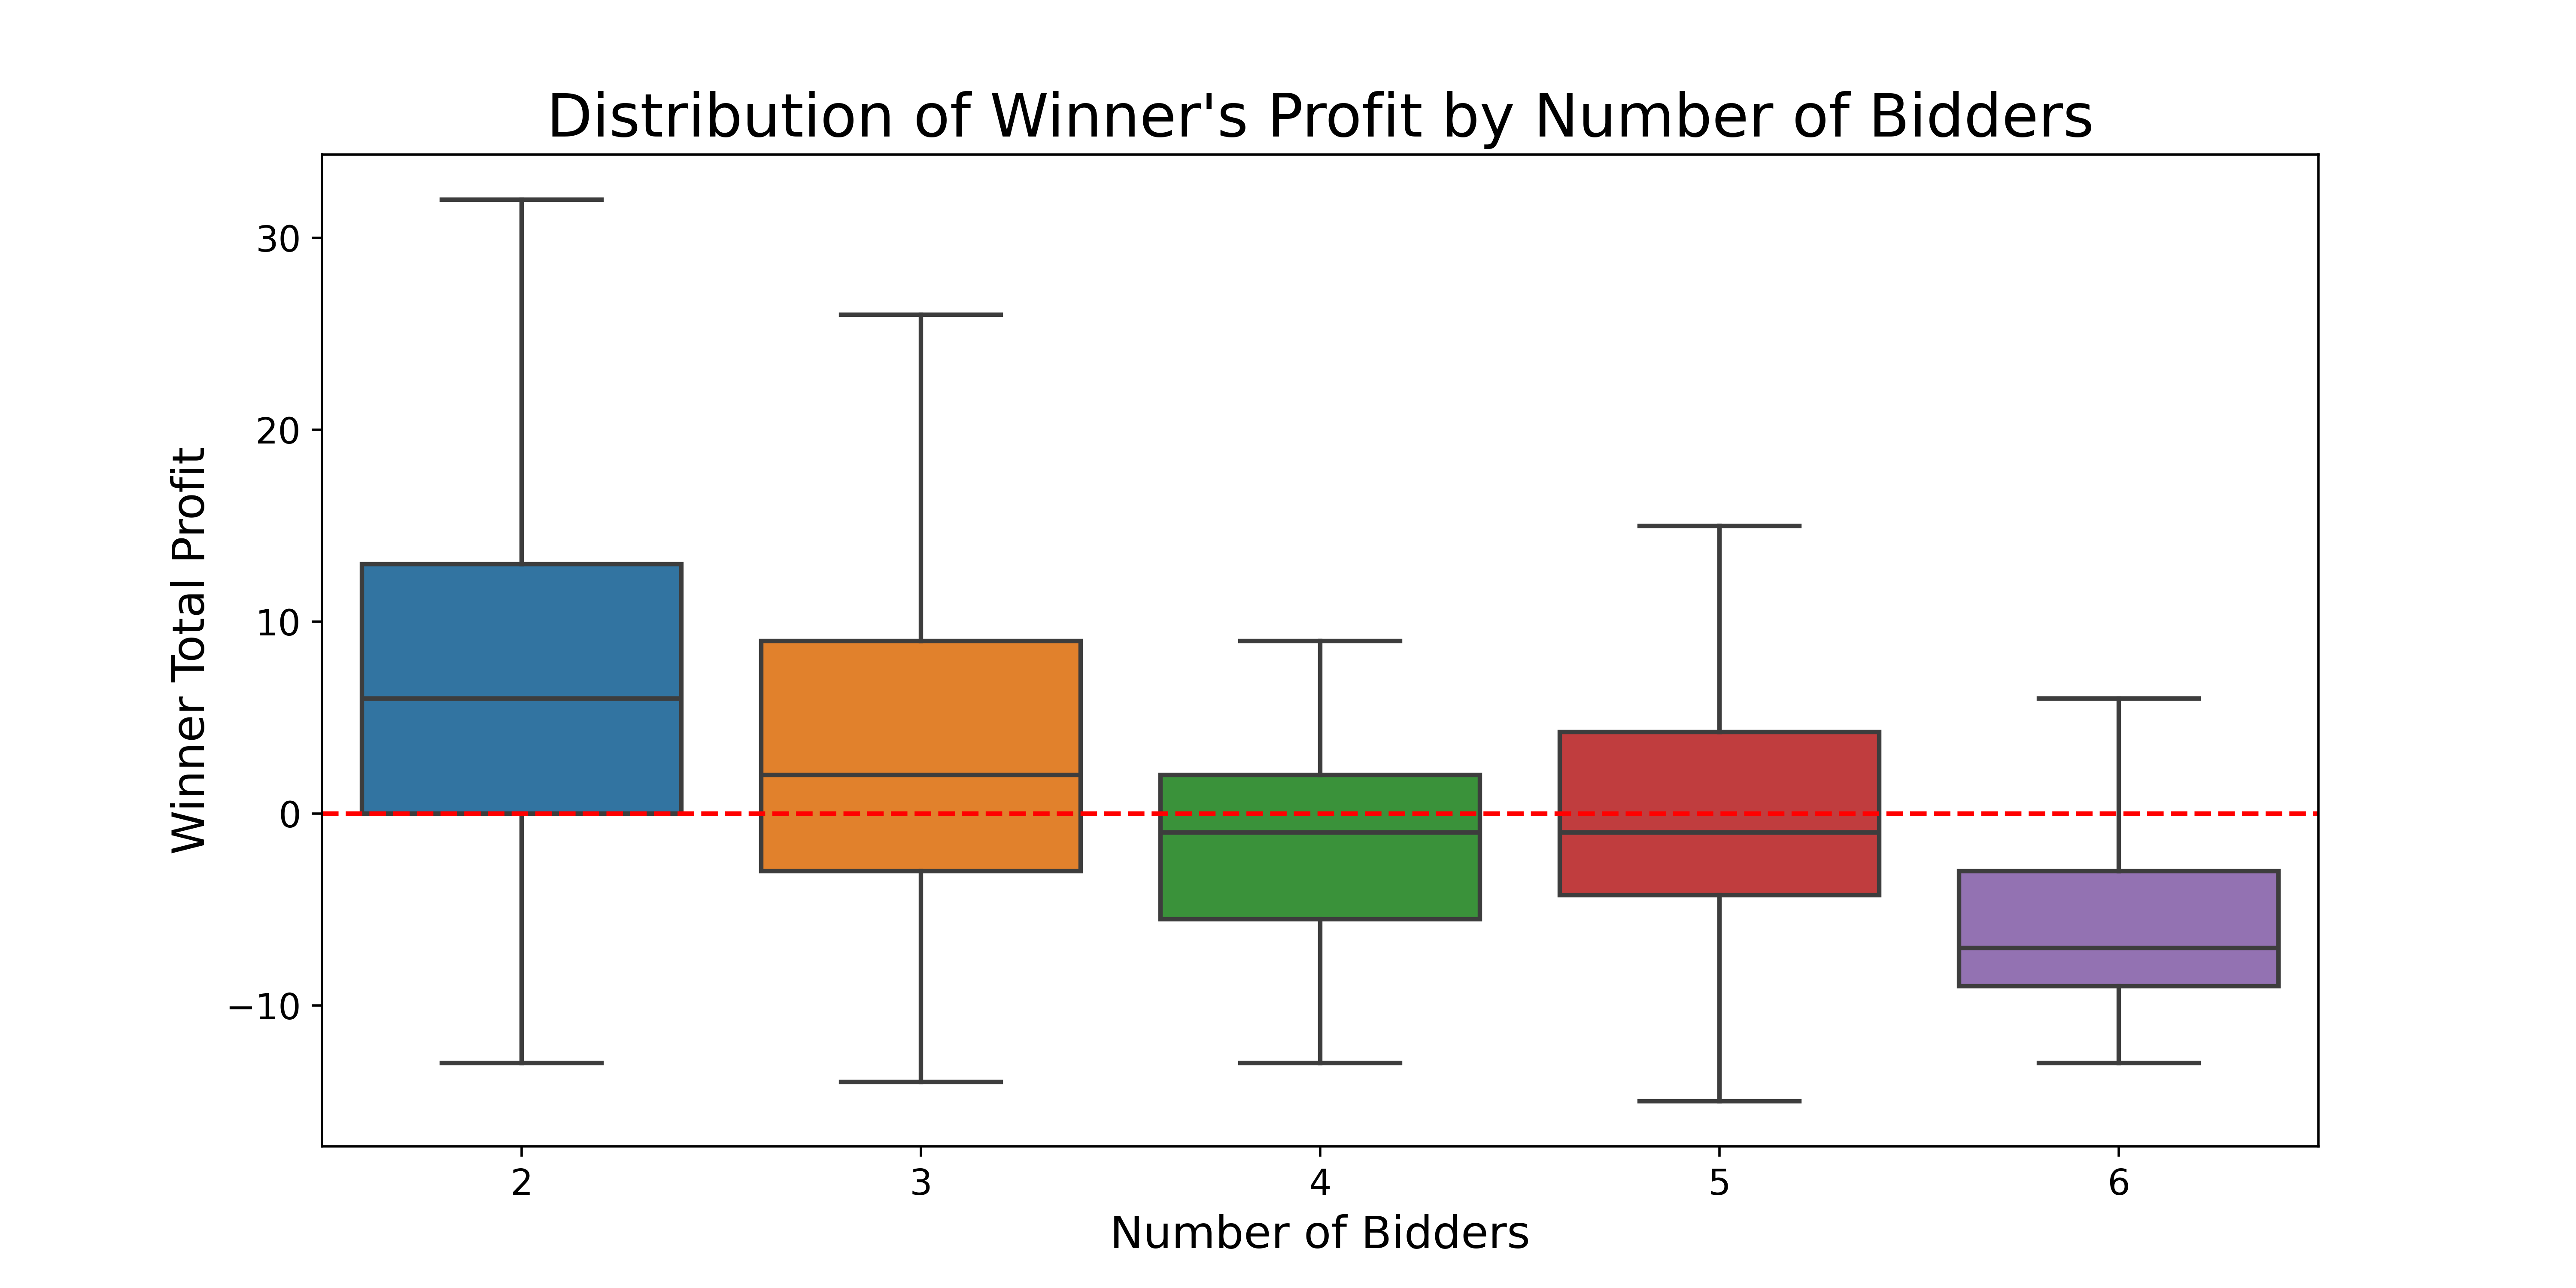
\includegraphics[width=\linewidth]{Figs/cv_plot.png}  % Adjust 'scale' as necessary to resize the image.
    \caption{\textbf{Distribution of the winner’s total profit across auctions with 2 to 6 bidders.} Each box shows the interquartile range of profits, with the median indicated by the central line. The horizontal red dashed line represents zero profit. As the number of bidders increases, the median winner's total profit decreases and more frequently turns negative. This echoes with the intensifying effect of the winner's curse in larger auctions.}
    \label{fig:winner}

\end{figure}


Our evidence suggests that LLMs play at about the level of experienced bidders, generally agreeing quite strongly with existing experimental results. 
However, `learning' remains a puzzle in this setting as well -- even when told the past history of play, agents don't learn to condition on the event that they win. 
A defense of LLMs here may be that this is just very hard: learning is non-trivial with human agents as well (in \citet{kagel1986winner} it takes players 15-20 periods to learn). 
This suggests more sophisticated learning techniques may be required to fully mitigate the winner's curse with LLM agents. 
It remains to see whether future generations of language models (e.g., GPT5, with better in-context updating and memory) fare better on this front, thereby shading optimally against the winner's curse.



% \subsection{Learning\TK{Comment for John: We're still not quite sure how to frame learning.}}
% In the next session, we will show the differences between these two agent queries.

% % This alternative prompt design provide a different data generation process.
% \textbf{Direct querying:} When using the Type \RNum{1} query, we found an almost static bidding behavior in all the auction forms for all agents.

% To further investigate into this, we queried agents' reasoning along with bids in a single LLM call. The following is a reasoning procedure for the first 4 rounds in a Second-price Sealed-bid Auction:

% \begin{enumerate}
%     \item Round 1: ``Given that my value for the prize is 40, I want to ensure that I make a profit if I win. By bidding 30, I leave room for a positive profit margin, even if the second-highest bid is close to my bid.''
%     \item Round 2: ``Given my value for the prize is 106, I want to bid high enough to have a good chance of winning but still leave room for a profit. By bidding 85, I hope to outbid my competitors while ensuring that the second-highest bid is low enough to make a profit.''
%     \item Round 3: ``Given that my value for the prize is 114, I want to bid high enough to have a good chance of winning but still leave room for a profit. By bidding 100, I hope to outbid my competitors while ensuring that the second-highest bid is low enough to make a profit.''
%     \item Round 4: ``Given that my value for the prize is 29, I want to ensure that I make a profit if I win. By bidding 20, I leave room for a positive profit margin, even if the second-highest bid is close to my bid. Additionally, since my value is relatively low, I prefer to bid conservatively in this round.''
% \end{enumerate}

% From the reasoning chain of the agent, we can find that the agent seems to follow a fixed template and rarely change its strategy over time. It always want to ``make some room for profits'' and ``outbid my competitors''. And from the behaviors, the LLM agent kept bidding \$10 to \$20 below its true value, leading to a stable negative deviation from its bids to values.

% \textbf{With Plan and Reflection:} Now with the additional steps on planning and reasoning, we found a more dynamical evolution of the strategies. For example, in the following case, the agent made an initial plan in the first round by trying a 50\% shading strategy and increasingly bid up to 100\% of the value.

% \begin{enumerate}
% \item Round 1: ``I will initially start with moderate bidding, around 50\% of my value, to gain data about competitors. Next, I will try aggressive bidding, almost 100\% of my value, to see if I can outbid others. Then, I'd adopt a conservative strategy, bidding less than 50\% of my value to minimise losses. Finally, I will formulate a dynamic strategy based on previous round deductions, adjusting bids according to competitors' behaviour. The aim is to learn how to maximise long-term profit considering the varying risk levels of each strategy. I'll adapt as necessary based on outcomes.''
% \item  Round 2: ``Based on previous round's data, I'll test an upward bidding strategy, starting from a 70\% value bid. My focus will be on winning, and learning how high other active bidders are willing to bid.''
% \item  Round 3: ``Marking an upward trend, my next strategy entails bidding near my value to explore winning potential. Depending on the highest bid, I aim to bid at approximately 90-95\% of my value, gauging aggresiveness of other bidders and analyzing their bidding behavior.''
% \item  Round 4: ``I plan to test a more aggressive strategy. I'll aim to bid near my value, approximately 90-95\% of it. I'll closely observe other bidders, particularly any patterns in their bids, to make informed future bidding decisions.''
% \end{enumerate}

% As shown in the Figure~ \ref{fig:learning}, there is a significant drop in the mean absolute deviation from bid to value in the first 4-5 rounds and stabilized since.


% \begin{figure}[h]
%     \centering 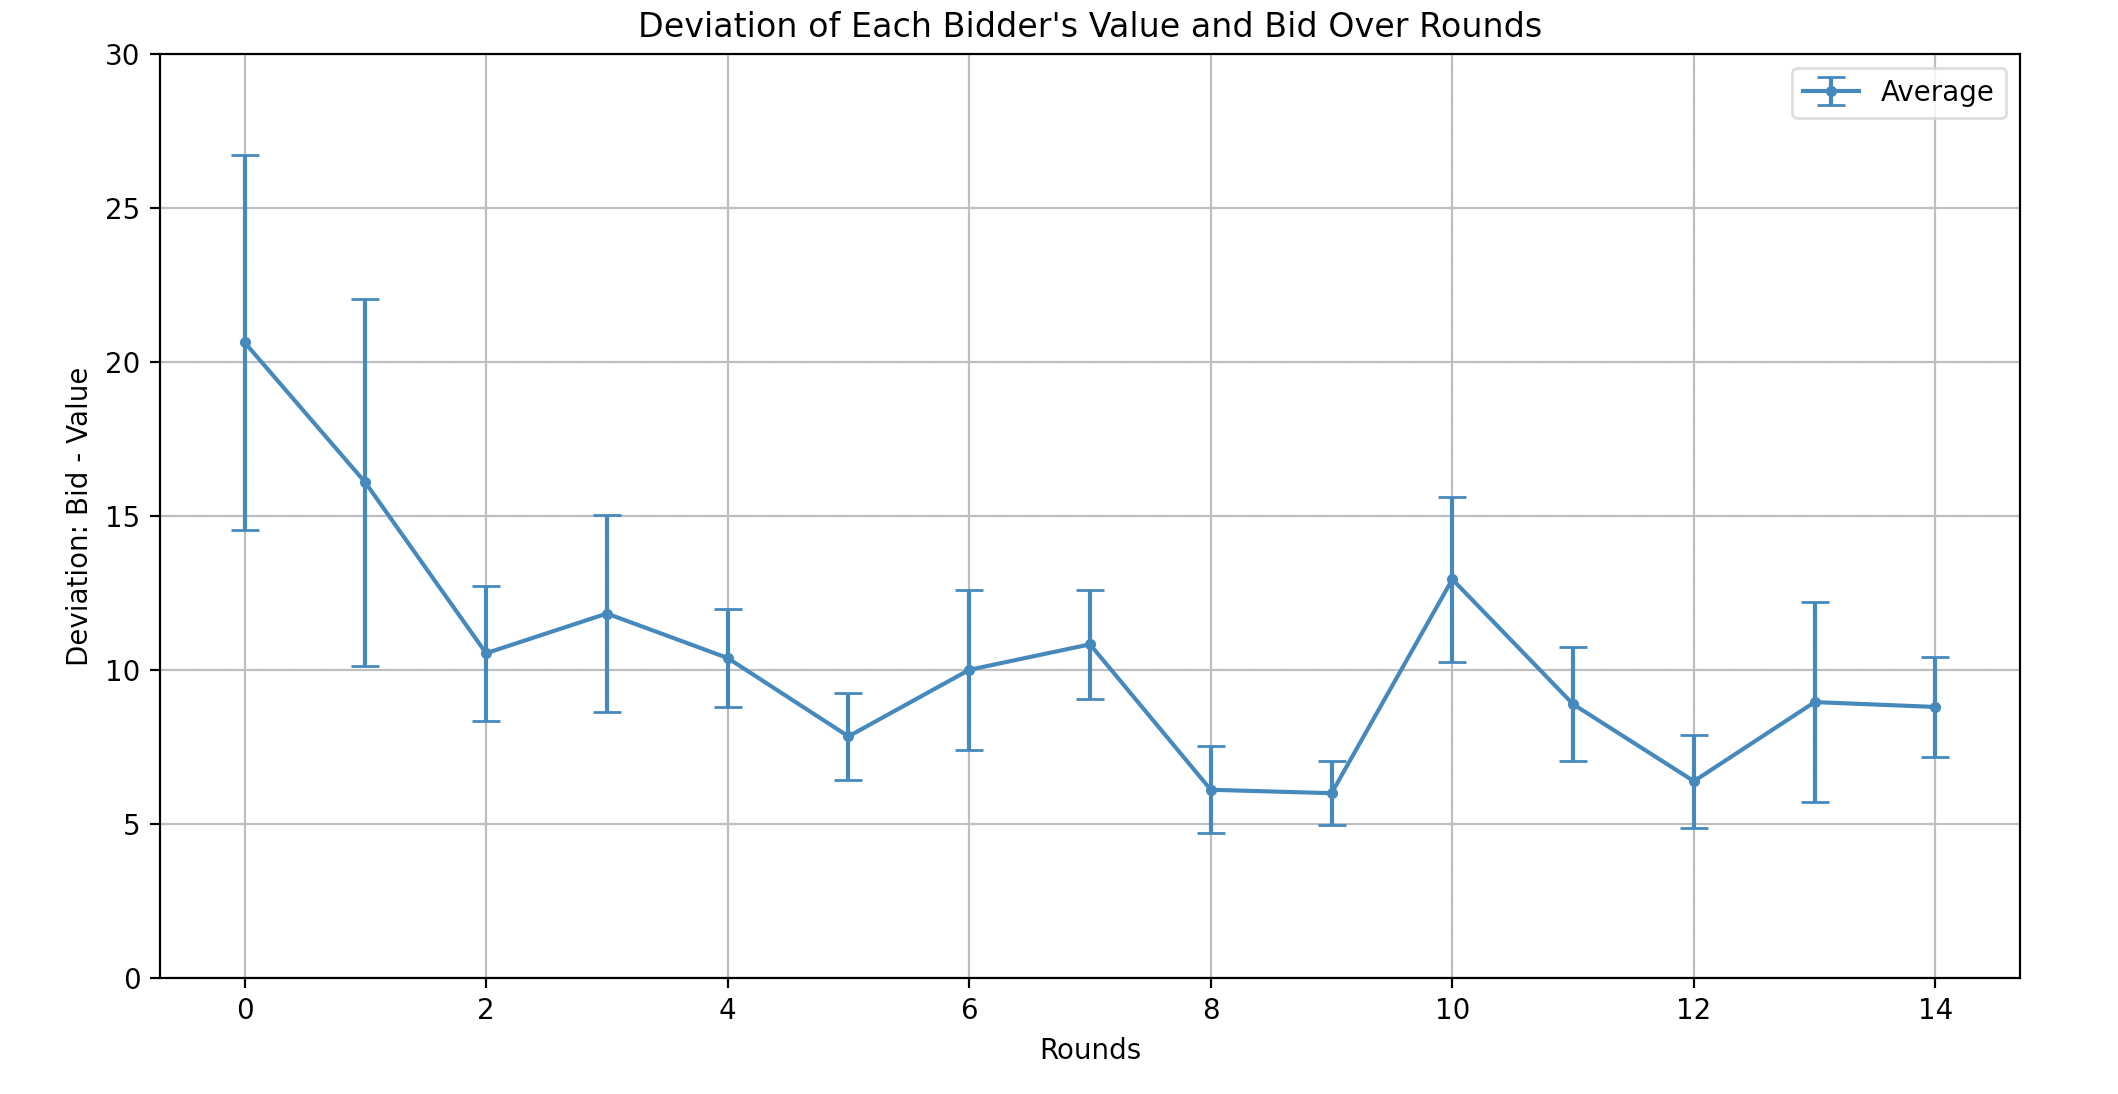
\includegraphics[width=0.7\linewidth]{Figs/learning.png}
%     \caption{\textbf{Agent learning over time} }
%     \label{fig:learning}
% \end{figure}


\section{New Empirics for Combinatorial settings}\label{session:combinatorial}
Finally, we considered multi-unit combinatorial settings -- namely auctions over complementary goods. 
The settings of combinatorial auctions is very rich but complex: various applications have required vastly different designs, with fruitful applications of the theory ranging from airport time slots to course allocations to spectrum auctions (\cite{rassenti1982combinatorial}; \cite{budish2011combinatorial}; \cite{milgrom2020clock}).

These examples highlight one difficulty with combinatorial auctions (CAs) in particular as the large design space -- diverse settings require different designs, making it difficult to obtain the data necessary to test promising mechanisms at scale before they're deployed.

Here, we applied our method to three formats of a typical CA. 
The generated data is used to compare the three formats, corroborating classic intuitions from mechanism design.

\subsection{Setting} In the multi-unit setting, there are 3 bidders in each auction, and bidders draw independent private values from a uniform distribution, $v \sim U[0, 99]$ for two goods, good $A$ and good $B$. 
Bidders observe the drawn values $v(A)$ and $v(B)$, and have superadditive valuation for the packages: $v(AB) > v(A) + v(B)$. 
In particular, we set $v(AB) = 2[v(A) + v(B)]$.
Bidders submit sealed bids for the goods and bids are processed according to the auction format. 
Here, we consider three different formats to auction items in this combinatorial valuation setting.
\begin{itemize}
    \item \textbf{Simultaneous single-item auction:} Each agent simultaneously submit a sealed bid for each item $A$ and $B$. The highest bidder for each good wins the good and pays their bid. \vspace{1mm}
    
    \item \textbf{Sequential single-item auction:} Bids are processed sequentially, first for good $A$ then for good $B$. The highest bidder for each good wins that good and pays their bid. Bidders first submit sealed bids for good $A$. Bidders are informed of the results of the auction over good $A$ before proceeding to the auction for good $B$. \vspace{1mm}
    
    \item \textbf{Single combintorial auction:} Bidders submit sealed bids for good $A$, good $B$, and the package $AB$. If the highest bid for package $AB$ is greater than the highest bid for good $A$ plus the highest bid for good $B$, package $AB$ is allocated to the highest bidder and they pay their bid. Else, good $A$ and good $B$ are allocated to their respective highest bidders, and the winners pay their bids. 
\end{itemize}

\subsection{Theoretical benchmarks}
The novel theoretical consideration in combinatorial environments comes from superadditive valuation when goods are complements -- in the sequential and simultaneous formats, agents may be willing to bid higher than their individual values for good $A$ or good $B$ in the hope of obtaining both goods and obtaining value $v(AB) = 2[v(A) + v(B)] > v(A)+v(B)$. 
Agents shade their bids to hedge against the risk that they only win one of the goods. 
This problem is worst in the simultaneous case, as in the sequential format, agents know whether they won good $A$ when submitting bids for good $B$ so bidding above $v(B)$ is strictly dominated. 
In the full combinatorial format where bids can be placed on bundles, agents should never bid above their valuation for either of the goods or the package, as their bid for a single good realizes only if they don't win the package.

With many goods, the winner determination problem for combinatorial auctions is also theoretically difficult and interesting \cite{lehmann2006winner}. 
We restrict our setting to two goods to avoid this difficulty for now.

\subsection{Simulation evidence}
Of the three auction formats tested in combinatorial settings, we found that the simultaneous auction (Figure ~\ref{fig:simu}) had the most overbidding for both goods. 

\begin{figure}[h!]
    \centering 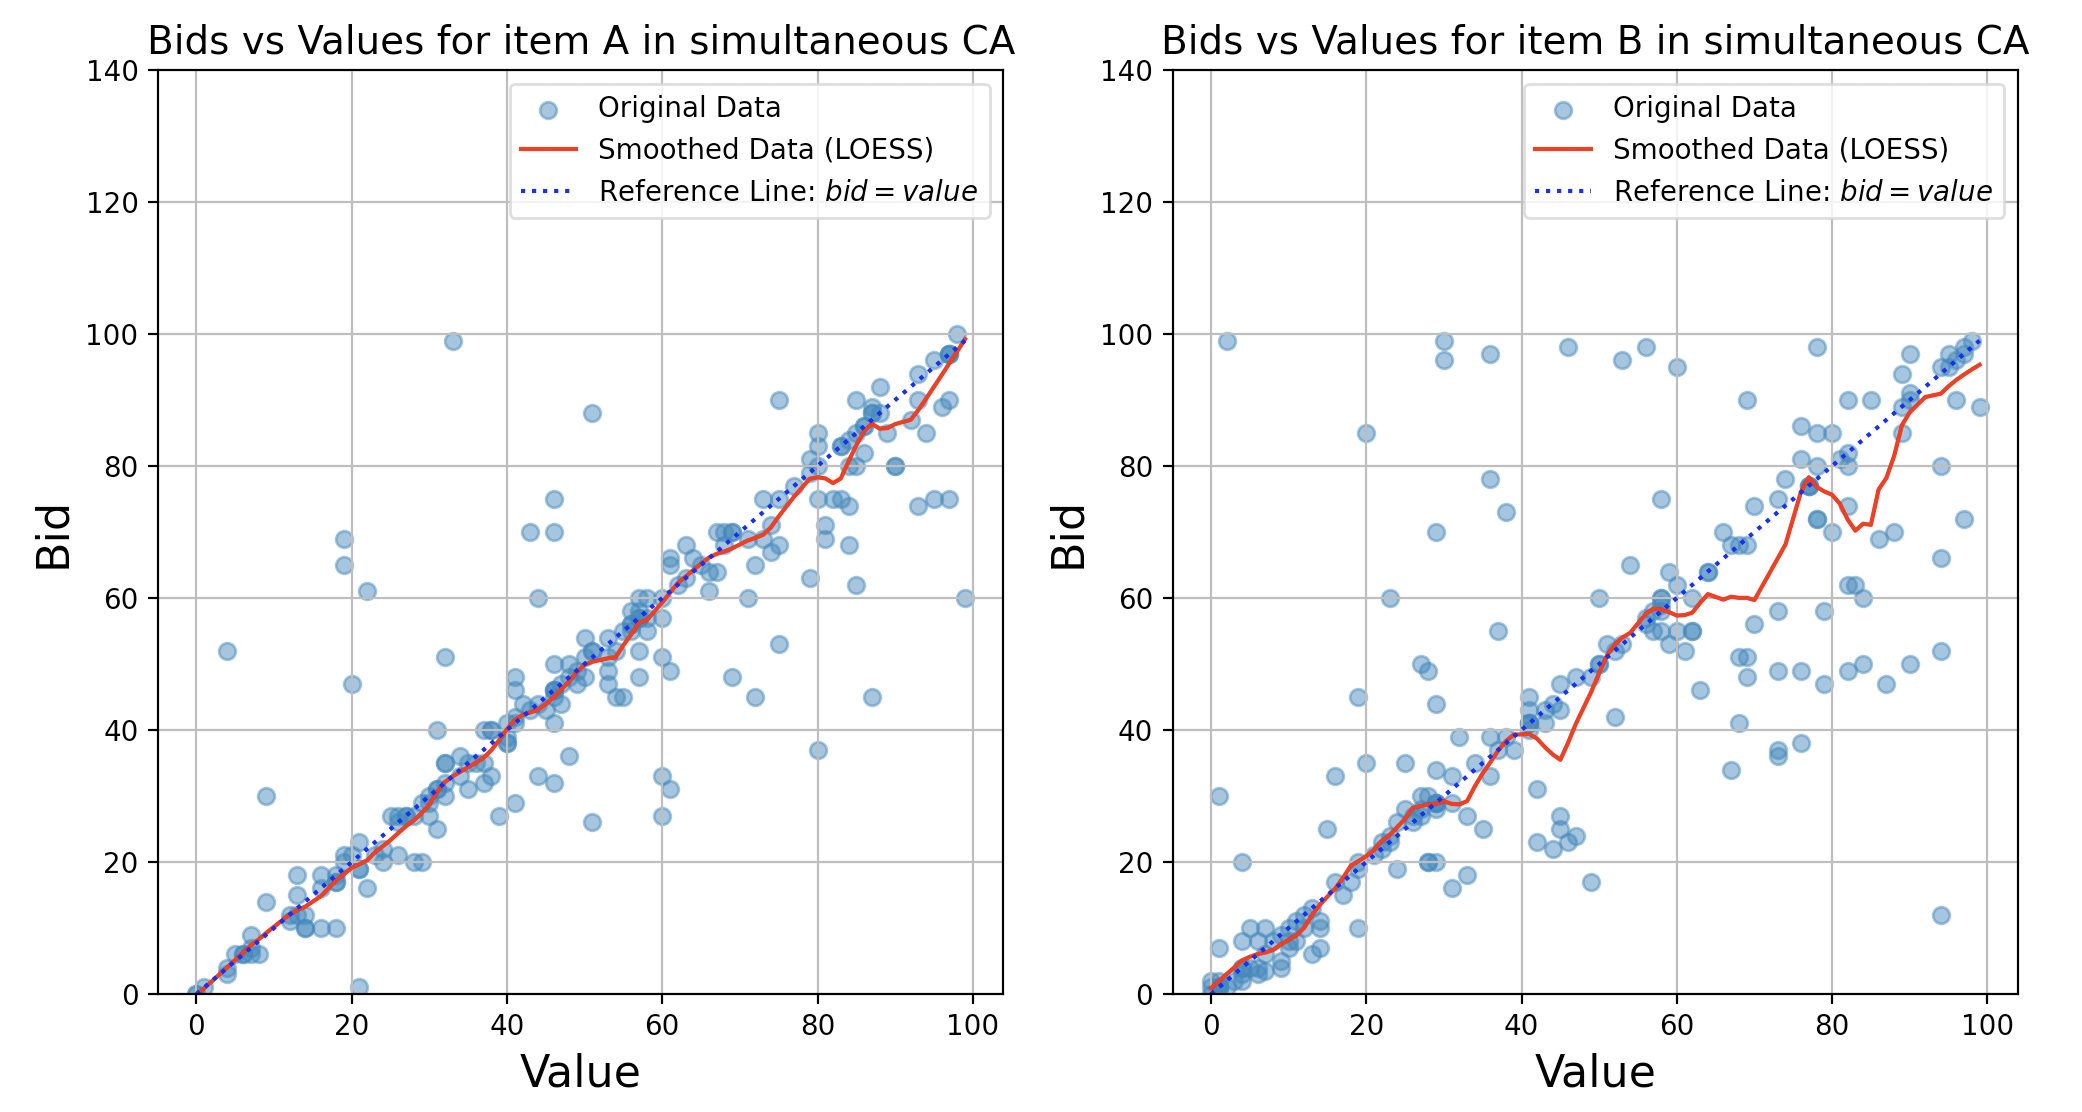
\includegraphics[width=\linewidth]{Figs/Simultaneous.png}
    \caption{\textbf{Simultaneous Combinatorial Auction} }
    \label{fig:simu}
\end{figure}

This corresponds to the theoretical intuition that agents, trying to capture both goods since this is very attractive under superadditive valuations, bid more than their value for a particular -- namely that the expected value of good $A$ for bidder $i$ is not just $v_i(A)$, but rather $v_i(A) + \mathbb{P}[\text{$i$ wins B}]\cdot(v_i(A) + v_i(B))$. 
However, the plots don't perfectly correspond to this theoretical benchmark, as overbidding in $A$ $(B)$ isn't monotonic in $v(A)$ $(v(B))$.


In striking contrast, in the sequential auction format (Figure ~\ref{fig:sequ}), we find that much more of the overbidding behavior in good $B$ is carried out by the \textit{ winners} of the first auction in good $A$. 
These are precisely the agents who benefit from superadditive valuations for package $AB$, suggesting that LLM agents conduct sophisticated play under complements. 
\begin{figure}[h!]
    \centering 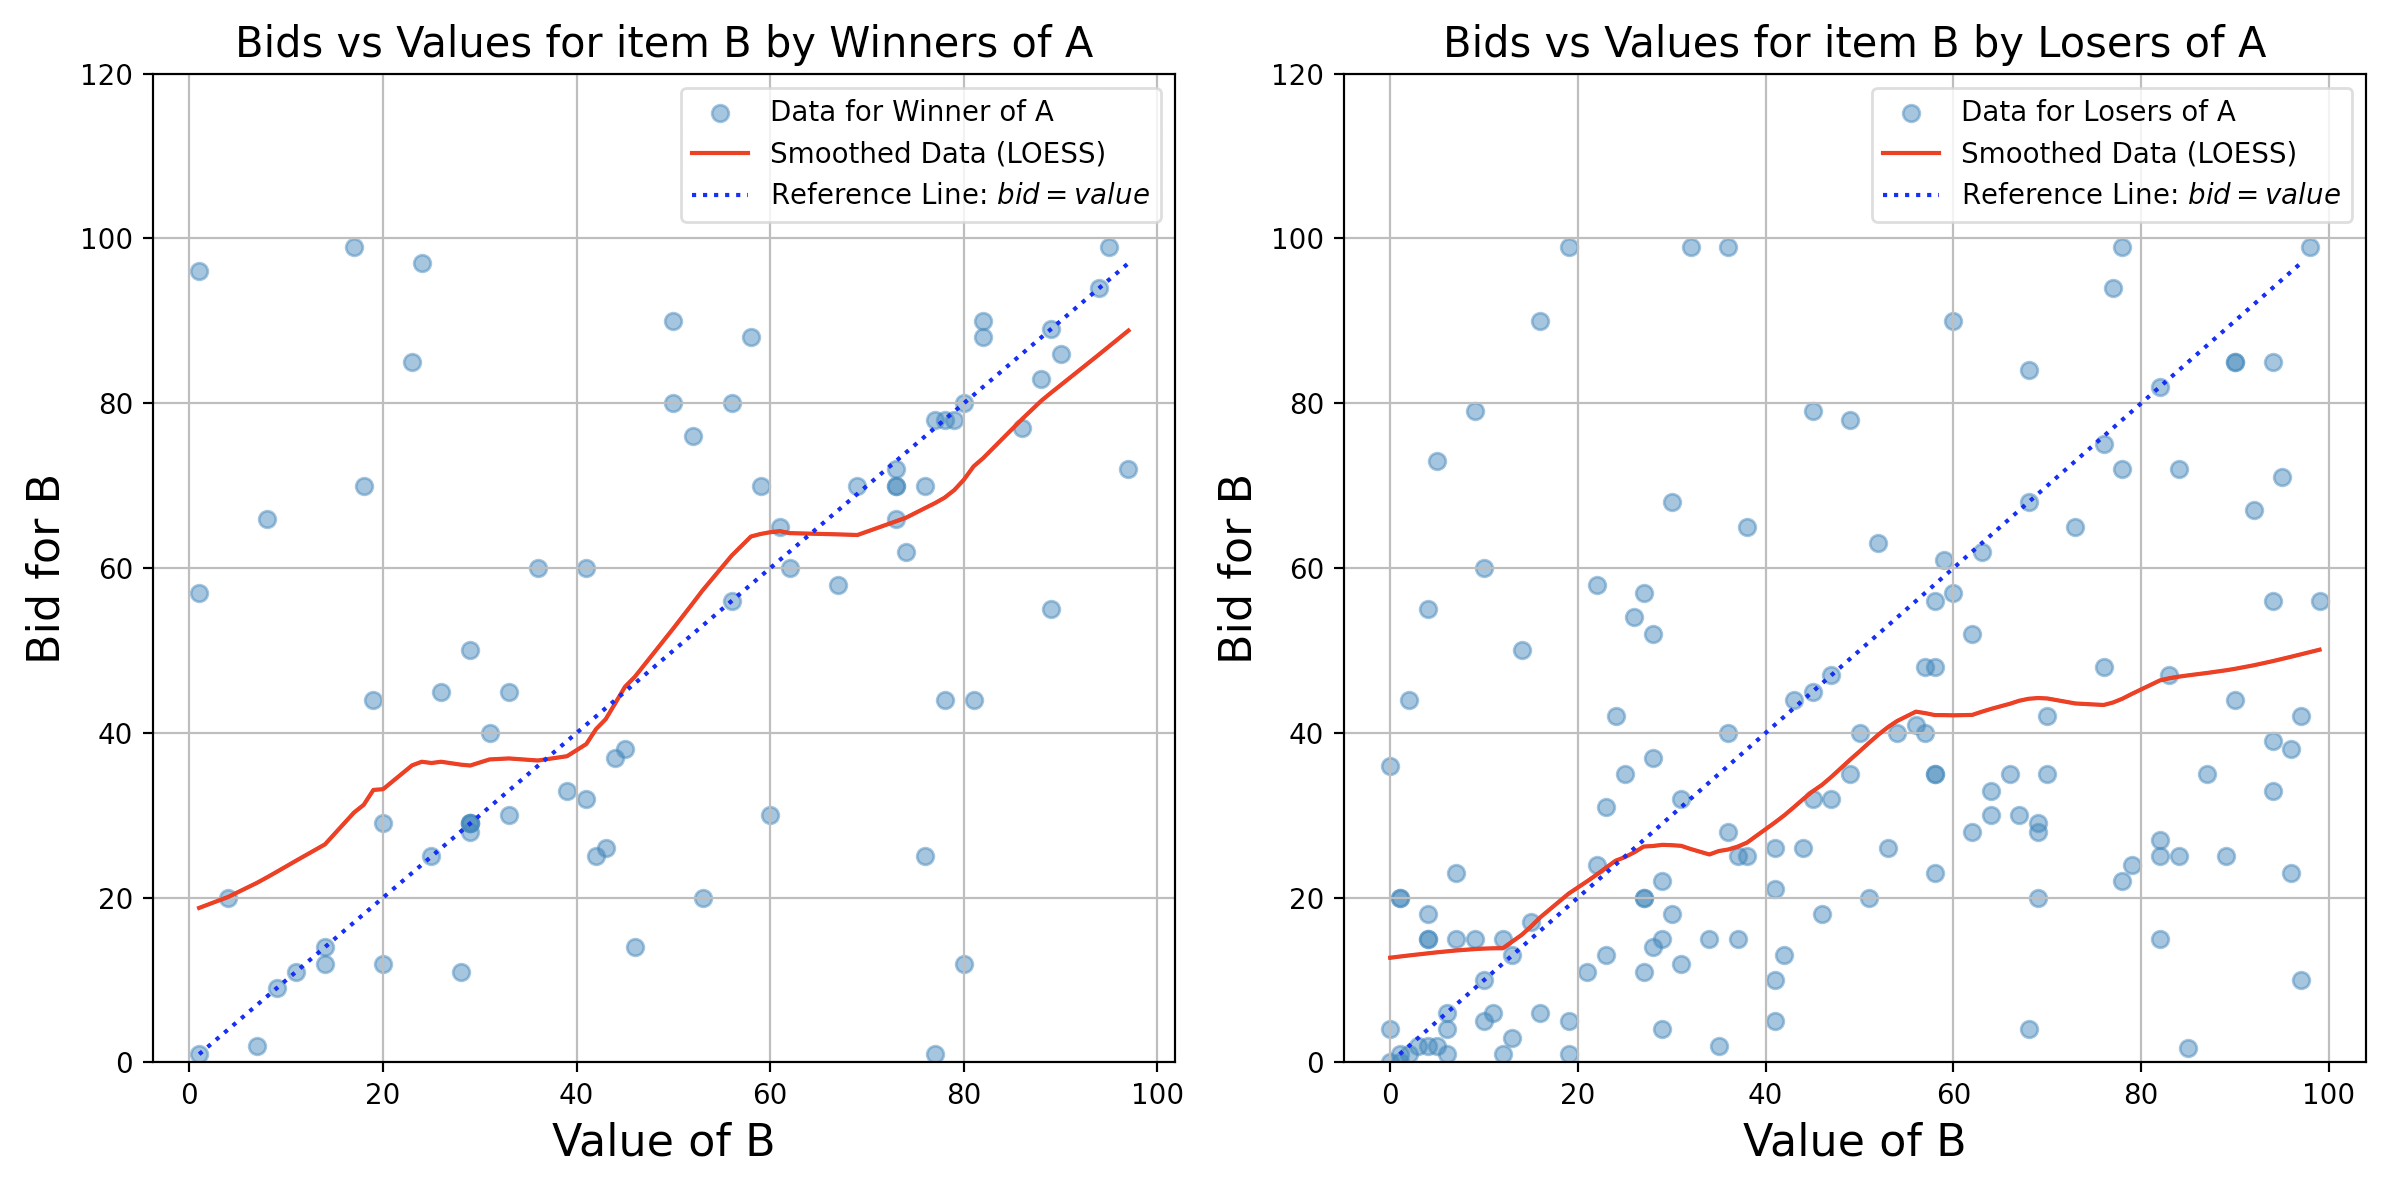
\includegraphics[width=0.9\linewidth]{Figs/Sequ.png}
    \caption{\textbf{Sequential Combinatorial Auction} }
    \label{fig:sequ}
\end{figure}

However, in comparison, LLM agents don't seem to play the general combinatorial auction as well (Figure ~\ref{fig:menu}). 
Recall that agents only pay their bid for (wlog) good $A$ if they win the auction for good $A$ but \textit{don't} win good $B$.
Hence, there should be no overbidding in the bids for individual goods. 
The LLM agents don't seem to bid in a way that appreciates this argument -- the plots below demonstrate some overbidding for both individual goods. 
In addition, there is also overbidding in the package auction, where the x-axis is the agent's package value $2[v(A) + v(B)]$. 
Future iterations of this work will hope to implement learning to observe if agents improve their play away from these mistakes over time.

\begin{figure}[h]
    \centering 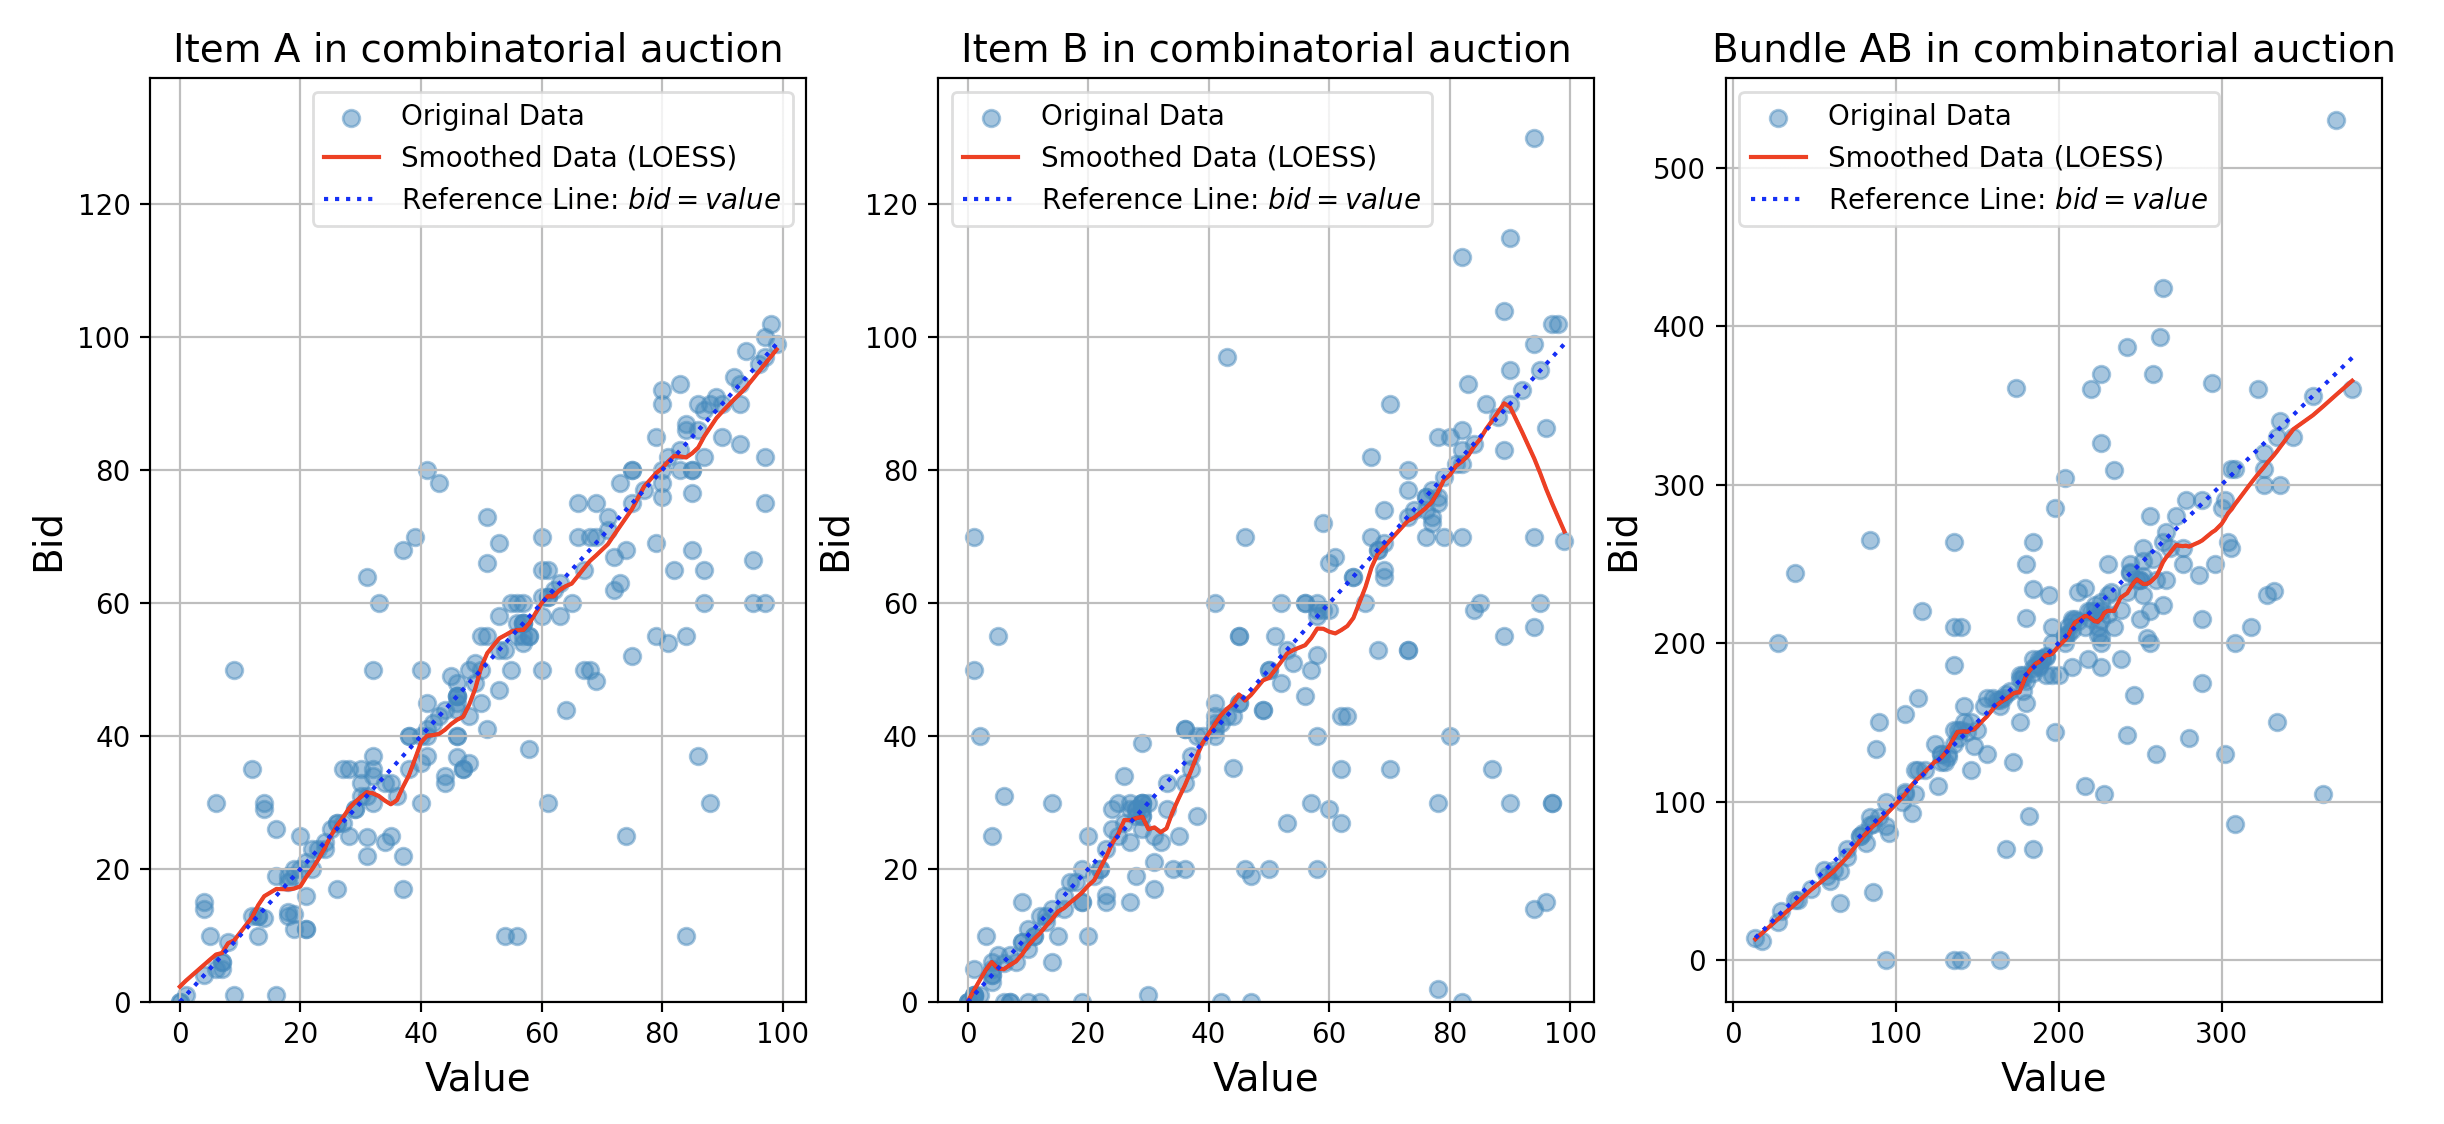
\includegraphics[width=\linewidth]{Figs/menu.png}
    \caption{\textbf{Menu Combinatorial Auction:} Bidders' value versus their bids for the item A, B and bundle AB. }
    \label{fig:menu}
\end{figure}


\begin{figure}[h]
    \centering 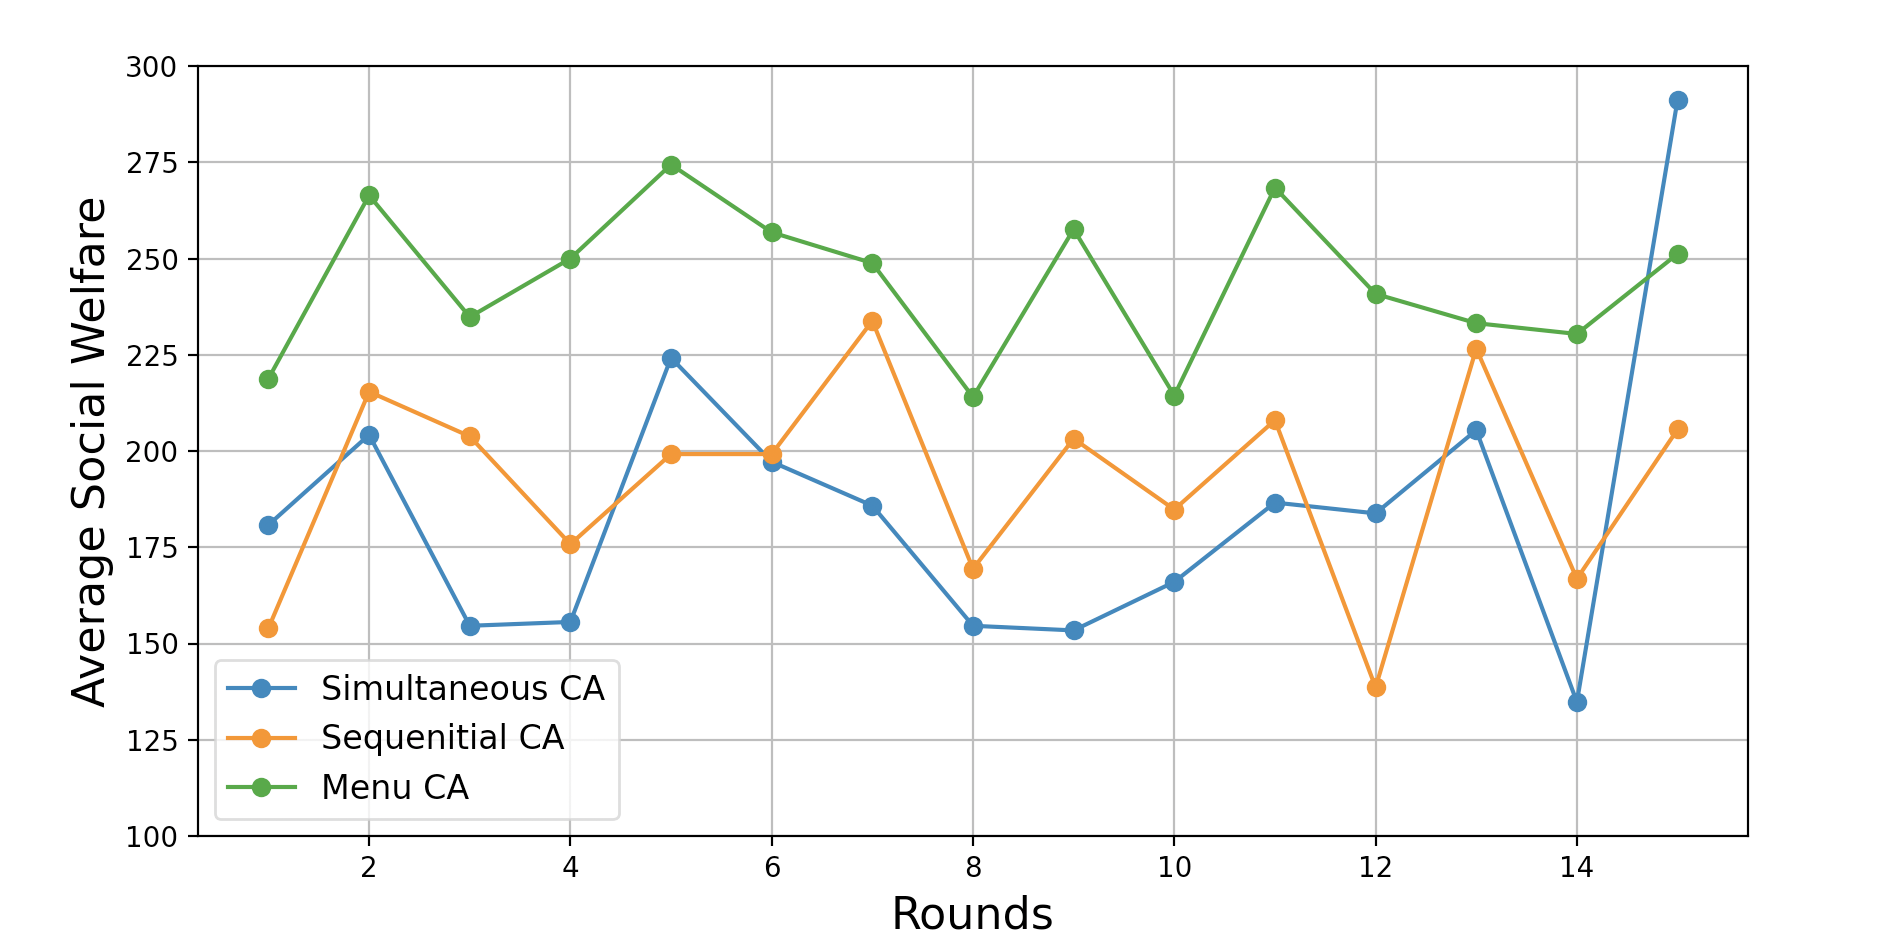
\includegraphics[width=0.9\linewidth]{Figs/social_welfare.png}
    \caption{\textbf{Comparison of social welfare in three Combinatorial Auctions} In all of the auction format, menu combinatorial format achieved the largest social welfare in almost every round. 
    And for most of time, simultaneous auction hit the lowest social welfare.}
    \label{fig:social}
\end{figure}

For measuring the efficiency for these multi-resource allocation scheme, we calculated the social welfare in each round as:
\begin{equation}
   S_i = 
   \begin{cases}
      2 \left( v_i(A) + v_i(B) \right) & \text{if } t_i(A) = t_i(B) eq 0\\
      v_i(A) + v_i(B) & \text{otherwise}
   \end{cases}
\end{equation}
As shown in Fig~\ref{fig:social}, In general, bidders retain the most surplus in the menu format and the least surplus in the simultaneous format. 
This is intuitive given agents have the greatest ability to plan in the menu auction.


\subsection{Case study:}
While we prompted agents to try out various plans in their pursuit for revenue maximizing bidding strategies, these combinatorial settings were the first in which agents actually experimented with strategies to learn. 

For example, in the sequential combinatorial auction, we observed price-correlation behaviors in the agents' planning.
\begin{quote}
    ``I'll bid approximately \$70 on item A to be more competitive. The outcome will inform my strategy for item B. If I win A, I'll bid aggressively (around \$73) on B to double my return. If I fail, I'll bid a conservative \$38 for B.''
\end{quote}

Planning documents maintained by LLM agents are rife with such long-term planning, suggesting an additional benefit of evidence from LLM agents: rich text data on convergence with learning in complicated games.


\section{Costs of generating synthetic vs. human data}
\TK{Hi John! Your feedback here would be very useful. 
Feels super fluffy but also like important discussion to have.}
% This paper investigates auction behavior through the lens of three distinct agents: {\em homo economicus} (theoretical predictions), real humans (existing empirical/experimental evidence), and {\em homo silicus} (simulated agents using large language models, or LLMs). 
LLMs and human labor have fairly different cost curves. 
LLMs are characterized by high upfront capital costs (eaten by companies like OpenAI and Anthropic) and extremely low marginal costs for individual tokens (passed on to consumers). 
In contrast, human labor costs for experiments are usually linear with minimal upfront costs, if not superlinear (the 5th hour of an experiment costs more than the 1st on a college campus). 
It's intuitive that, insofar as most of the capital costs of developing the LLMs aren't being passed on to us researchers, LLMs are much cheaper for data generation purposes than humans are.

In the context of this paper, LLM agents reduced costs relative to human experiments by around three orders of magnitude. 
The lab experiments cited in \cite{li2017obviously} with 404 human participants cost over \$15,000, while the same experiments with LLM agents costs us about \$10 to run. 
Additionally, the original experiment had 3 phrases and cost the researchers over 3 years to collect data -- design, implementation, and administration costs are not reflected in the \$15,000 final ticket, and for the best researchers, the opportunity cost of this time is even more expensive.

Finally, while LLMs are likely much cheaper for generating types of data we are comfortable with, they also enable data processes that would be prohibitively costly in the real world. 
We've outlined several such reasons below.

\begin{enumerate}
    \item \textit{Keep agents around}. Ad auctions have been a mature industry for nigh on two decades, with the core host of players in each sub-industry being fairly stable. 
    Suppose Google, two decades ago, was trying to decide whether to use the GSP or Vickrey design to sell ads in a complicated combinatorial setting. 
    Google has the resources to run extensive internal experiments to inform design, and yet even Google cannot hold the leading ad sellers on their platform in retainer for a decade to generate data on longterm outcomes under a particular mechanism.

    As designs get more complicated, theory becomes less predictive. 
    Unforseen frictions such as market power or information asymmetries may play large roles in the health of a market after its design has been locked in.

    LLMs enable fast and cheap experimental revolutions, enabling us to learn something about play over the span of decades with the same set of agents. 
    We cannot do this with human experiments.

    \item \textit{Play with experts.} Auctions in the hands of economists are beautiful, mathematical objects. 
    In applied settings, good auction play often relies crucially on institutional details and industry knowledge. 
    It costs a lot to teach experimental subjects the knowledge required for them to play an auction in context. 
    However, it's cheap to tune an LLM expert -- once you train one effectively, you've trained them all.

    \item \textit{Expand the design space.} Experiments with human participants have impacts in the real world, and as such, we as a society place constraints on the design space for experiments. 
    LLMs, however, have a much weaker constraint in this regard -- they can be used to learn from experiments that small research budgets or IRB would not allow. 

    Consider the design of a spectrum auction at the level of a large country. 
    To keep participants sincere, we'd like to provide incentives -- but providing these incentives is impossible given reasonable IRB restrictions and research budgets.
    Seeding expert LLMs to play with the sophistication of a hedge fund may offer some empirical insight into how the mechanism fares in the real world.

    % even if we could provide incentives on the order of the final stakes (billions of dollars), it would be infeasible to implement the experiment in the real world. Moving billions of dollars to telecom companies and hedge funds would 1) permanently change the setting of the auction, thereby perhaps requiring new design; 2) be a gross misuse of tax dollars; and 3) 

    \item \textit{Cheap textual data.} Even if you could run experiments at scale with the desired experts, seeing inside their minds is an entirely different endeavor.
    Consultants are expensive and sincerity doubly so. 
    LLMs, however, endowed with learning capacities as with chain-of-thought techniques, can be enabled to produce just such data.

    In fact, as demonstrated in this paper, LLMs can generate quality textual evidence (both while planning strategy in the mechanism and after playing the mechanism) to supplement researcher analysis. 
\end{enumerate}

% \subsection{New methods:}

% Compared with real human lab experiment, our paper offer new way for fast iteration.

% The richness of text-based responses revealed more information than a typical number-based lab experiment.

% When asked the LLM-participants to make a decision, we can effortlessly add a query module for their reasoning without the risk of causing harms to the human subjects



\section{Conclusion}
This paper reports the results of more than 1,000 auction experiments with LLM agents. 
In particular, we find behavior that conforms with important experimental results (i.e., evidence of risk-averse bidding, evidence that clock auctions are `easier' to play, and evidence for the winner's curse in common value settings). 
We also test theoretical intuitions for combinatorial design in a novel way, generating experimental evidence for three classic CA formats. 
Though the results are encouraging, we see this work as preliminary,
primarily putting forward a framework on how to think about LLM experimental agents as proxy for human agents.
 In particular, the design space for prompting is large, and we hope that interested readers
 will use our code to run simulations testing their own prompt variations. 
 \TK{John: should we make the conclusion more punchy?}

In addition, while this paper focuses on auction theory, future work may use LLM sandboxes to test other  kinds of
economic mechanisms (e.g., voting, matching, contracts, etc.). 
As techniques are developed to validate LLM models as proxies for human behavior, they can be used to obtain what would otherwise be prohibitively expensive evidence. 
As a provocative example, while ethical and financial constraints make it impossible to run voting experiments at the scale of nations, it may be possible to run such experiments with LLM agents. 

This paper acts as a proof of concept for LLMs as human proxy agents. 
Our primary motivation is to  use LLM agents to inform novel
economic design. 
Some auction formats, such as combinatorial auctions, are complex and can be  particularly difficult to run frequently and at scale in traditional lab experiments. 
Augmenting these traditional lab experiments with LLM experiments, when correctly validated, may open up wide new avenues 
to better understand the design tradeoffs in these kinds of complex and often high-stakes environments.


\subsubsection*{Acknowledgments}
We thanks EDSL and Robin Horton for techical support in building LLM agents.


% \bibliography{iclr2024_conference}
\bibliography{llm_auction}
\bibliographystyle{iclr2024_conference}

\appendix
\section{Appendix}

\subsection{Bidding without planning and reflection}

For a comparison, we can query the LLM's decision directly after informing them about the auction rules and the current value (Off-the-box agent). 

We repeated the experiment for SPSB and FPSB auction under IPV setting. 
The overall results are similar.

\begin{figure}[h]
    \centering 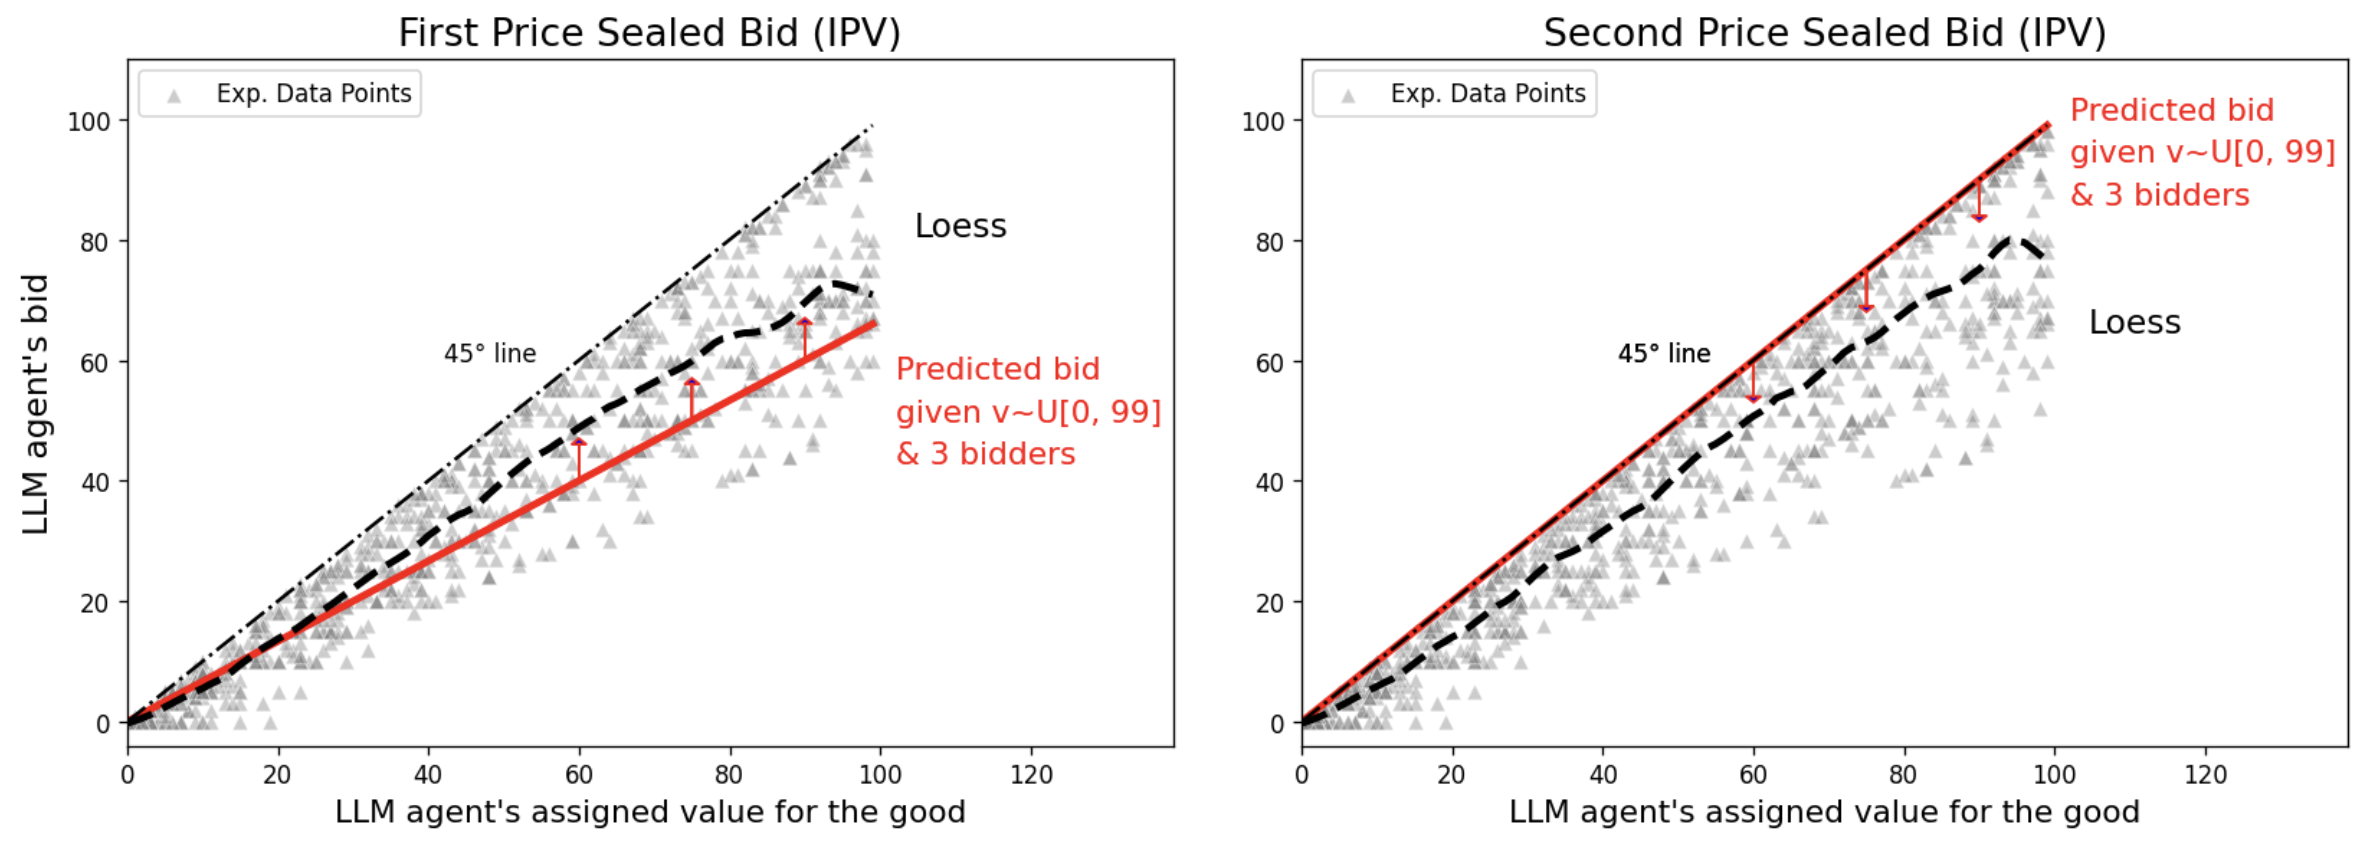
\includegraphics[width=\linewidth]{Figs/FPSB_off-box.png}
    \caption{\textbf{ Off-the-Box agent in FPSB and SPSB under IPV setting.} }
    \label{fig:fpsb}

\end{figure}
\end{document}
